% For printing in a4
%\documentclass[a4,10pt,twoside,openright,italian,english]{book}% twoside!

% For printing with the A5 format
\documentclass[10pt,twoside,openright,english,italian]{report}% twoside!

% Set paper size
\usepackage[twoside=true]{geometry}

%For printing with the weird format
%\geometry{
%	paperwidth=17cm,
%	paperheight=24cm,
%	margin=2cm,
%	top=2.3cm,
%	bindingoffset=0.4cm
%}
% For printing in a4
\geometry{a4paper,
  margin=3cm,
  top=3.8cm,
  bindingoffset=0.4cm
}




%Uncomment this for final prints: this just enables printing on a4 paper
\usepackage[cam,center,a4,pdflatex,axes]{crop}
% See https://en.wikibooks.org/wiki/LaTeX/Internationalization
\usepackage[english, italian]{babel}

\selectlanguage{english}
\title{First Person Shooter level generation using Generative Adversarial Networks}
\author{Edoardo Giacomello}


\usepackage{hyperref}
\hypersetup{
	colorlinks=true, %set true if you want colored links
	linktoc=all,     %set to all if you want both sections and subsections linked
	linkcolor=black,  %choose some color if you want links to stand out
}

\usepackage{fancyhdr}

\fancyhf{}
\fancyhead[LE]{\nouppercase{\makebox[0pt][r]{\thepage\hspace{.1in}}~\leftmark}}
\fancyhead[RO]{\nouppercase{\rightmark~\makebox[0pt][l]{\hspace{.1in}\thepage}}}
% redefine cleardoublepage so it won't insert an header
\makeatletter
\renewcommand*{\cleardoublepage}{\clearpage\if@twoside \ifodd\c@page\else
	\hbox{}%
	\thispagestyle{empty}%
	\newpage%
	\if@twocolumn\hbox{}\newpage\fi\fi\fi}
\makeatother

\usepackage[backend=bibtex]{biblatex}
\addbibresource{bibliography.bib}



\usepackage[toc]{glossaries}
\makeglossaries

\usepackage{tabularx}
\usepackage{multirow}
\renewcommand\tabularxcolumn[1]{m{#1}}% for vertical centering text in X column
\usepackage{enumitem} % For managing lists
\setlist[enumerate,itemize]{ % apply settings globally 
	wide=\parindent,
	topsep=3pt,
	partopsep=0pt,
	parsep=0pt,
	itemsep=2pt
}
\usepackage{graphicx, caption}%
\graphicspath{{figures/}}


\begin{document}
	
	%TODO Fix the headings
	\maketitle
	\cleardoublepage
	\pagestyle{fancy} 
	\normalfont
	\chapter*{Abstract}
\addcontentsline{toc}{chapter}{Abstract}
%
This work studies the feasibility of level generation for First Person Shooter games using Generative Adversarial Networks in the setting of Procedural Content Generation via Machine Learning (PCGML).
As the Procedural Content Generation becomes a widely used technique in developing video-games, many researchers explored new paradigms for generating game content based on generative models that learn from existing content. So far, few work has been done in applying these novel techniques to games that allows a two-dimensional exploration of the levels rather than a one-directional traversal that is typical of platform games. Our study proposes as a starting point in applying Generative Neural Networks to the problem of generating this type of two-dimensional levels, using DOOM as our sample game. 
In this work, we first expand the existing Video Game Level Corpus proposing a dataset of 9000 DOOM levels collected from the community and we design a system for extracting a set of features and representing the levels as images and tiled representation. We then introduce some of the main issues in applying existing techniques to this particular domain, selecting a set of measures that help in assessing the perceived sample quality in our case. We train two different models which differ from the presence of input features and we design a set of experiments to evaluate the impact of the input features on the generated levels. In addition, we study the possibility of controlling the level generation by acting on the network inputs. Our results show the advantages of adding the level features as a network input from both the point of view of sample quality and learned feature distribution, indicating our method as a viable option for being utilized as an automatic tool for level generation which doesn't require particular domain expertise.

\chapter*{Estratto in lingua Italiana}
\addcontentsline{toc}{chapter}{Estratto in lingua Italiana}
\selectlanguage{italian}

Questo lavoro analizza la fattibilit\`a della generazione di livelli per videogiochi "Sparatutto" utilizzando le Reti Antagoniste Generative (GAN), nel contesto della Generazione Procedurale di contenuti attraverso l'apprendimento automatico (PCGML).
Con la crescente applicazione di tecniche di Generazione Procedurale nell'industra videoludica, molti ricercatori stanno esplorando nuovi paradigmi per generare nuovi contenuti utilizzando modelli che apprendono da contenuto pre-esistente. Fino ad ora, poco \`e stato realizzato in merito all'applicazione di questo nuovo paradigma a giochi che permettono un'esplorazione bi-dimensionale dei livelli, in contrapposizione al classico attraversamento monodirezionale tipico dei giochi "Platform". Il nostro studio si pone come punto di partenza per l'applicazione delle Reti Antagoniste Generative al problema della generazione di questo tipo di livelli bi-dimensionali, in particolare utilizzando il gioco DOOM come riferimento.
Come primo passo, proponiamo un dataset di 9000 livelli di DOOM collezionati dalla comunit\`a di videogiocatori in aggiunta a quelli gi\`a forniti dal Video Game Level Corpus, progettando un sistema per estrarre automaticamente un insieme di caratteristiche descrittive dei livelli e convertire gli stessi in immagini. Proseguiamo selezionando un insieme di misure che agevolano la valutazione oggettiva della qualit\`a dei livelli generati, evidenziando le principali difficolt\`a nell'applicare le tecniche esistenti al nostro dominio applicativo. Ottimiziamo quindi due reti diverse, che differiscono per la presenza in ingresso delle caratteristiche dei livelli e definiamo un insieme di esperimenti per valutare l'impatto che gli input aggiuntivi hanno sulla generazione dei livelli. Inoltre, analizziamo la possibilit\`a di controllare la generazione dei livelli agendo sugli input aggiunti alla rete. I risultati ottenuti mostrano i vantaggi dell'aggiunta delle caratteristiche dei livelli come input alla rete, sia da un punto di vista della qualit\`a dei campioni generati che dalle distribuzioni apprese, indicando che il nostro metodo pu\`o essere utilizzato come una opzione valida per generare livelli senza la necessit\`a di particolare esperienza nel dominio applicativo.
 




\selectlanguage{english}


	\cleardoublepage
	%\large
\begin{flushright}
\itshape{ A Cristina, per avermi sempre supportato e dato i giusti consigli.} \\*
\itshape{ A mio padre, per avermi sempre insegnato ogni cosa.} \\*
\itshape{ A mia madre, per tutto ci\`o che fa.} \\*
\end{flushright}

	\cleardoublepage
	\chapter*{Acknowledgments}
\addcontentsline{toc}{chapter}{Acknowledgments}
	\cleardoublepage
	%%%%%%%%%%%%%%%%%%%%%%%%%%%%%%%%%%%%%%
% TOC
%%%%%%%%%%%%%%%%%%%%%%%%%%%%%%%%%%%%%%
\tableofcontents
\cleardoublepage


\listoffigures
\cleardoublepage


\listoftables
\cleardoublepage

	\cleardoublepage
	\chapter{Introduction}
%TODO: Some description
\section{Background: Level Design}
%% Parla dei principali problemi del level design, di quanto sia laborioso per un designer creare livelli interessanti
\section{State of the Art}
\subsection{Procedurally Generated Content}
% Parla della storia del PGC e di come si sia proposto come soluzione al problema del design
\subsection{Procedural Content Generation via Machine Learning (PCGML)}
% What is proposed from snodgrass at al
\section{Scope}
% Si vuole proporre un modello alternativo che in linea teorica dovrebbe portare alcuni vantaggi rispetto al PCG, ovvero un approccio basato su machine learning applicato a DOOM, che permette di aiutare il designer non solo nel processo di generazione dei livelli ma anche nel sfruttare caratteristiche intriseche nei dati senza una esplicita definizione delle stesse da parte di un esperto (questo al costo di una certa quantità di dati da analizzare). Si vuole descrivere un sistema (...) ed evidenziare le principali problematiche incontrate e le motivazioni per cui questi problemi non sono affrontabili con le tecniche in uso correntementente.
\section{Thesis Structure}
\section{Summary}
	\cleardoublepage
	\chapter{Towards learn-based level generation}
\paragraph{Overview} The scope of this chapter is to further describe the setting of our work and highlight the main differences between the work that have been currently done in the literature and the one we introduce in the following chapters. In particular, section~\ref{sec:gantheory} first provides the theoretical background necessary to understand the setting in which our work take place. Then, section~\ref{sec:doominfo} describes and motivates the choice of the game we work with. Lastly, section~\ref{sec:considerations} reveals some important considerations about the setting just described and the possible difficulties in this type of research.
%TODO: Bisogna anche sottolineare la congiunzione tra ML e PGC, che ha originato questa tesi
\section{Generative Adversarial Networks}
\label{sec:gantheory}
\subsection{Overview}

\label{sec:introgan}
\paragraph{GAN} A model that in the latest years gained increasingly more interest in the field of Machine Learning research is the one of the Generative Adversarial Network, proposed by \citeauthor{gan} in \citetitle{gan} (\citeyear{gan}) \cite{gan}. The main idea of this kind of generative model is to use two neural networks which are posed in an adversarial setting that models a two-player Minimax Game \cite[p.~276]{minimax}. In particular, a generative network called G is trained to capture the data distribution while a discriminator network D estimates the probability that each sample comes from the real data distribution rather than the one generated by G.
\paragraph{Conditional GAN} In our work we make use of a modification of the GAN model introduced by \citeauthor{conditionalgan} \cite{conditionalgan}, which allows to condition the data generation to class labels. This structure is summarized in section \ref{sec:modelstructure} where the logical structure of the generative model we adopt is presented.

\paragraph{Additional Architectures} Due to the amount of interest that \glspl{gan} have raised, many researches have been conducted to improve the quality performances of \glspl{gan}, leading to a variety of proposed new architectures. They can be classified as modifications to the underlying neural network architectures or even to the conceptual setting of the model itself, by means of changes to the loss function or the training algorithm. Other, less formal but still effective adjustment to the proposed models are the so called "tricks" in machine learning discussion communities, which adoption is often suggested in order to improve the difficult training of the network. The final architecture adopted is described in section \ref{sec:networkarch}.


\subsection{Deep Convolutional GAN}
\subsection{Wesserstein GAN}
\subsection{Wesserstein GAN with Gradient Penalty}
\section{Game of choice: DOOM}
\label{sec:doominfo}
\subsection{Description}
\subsection{Motivation}
% Parla del game engine, dei livelli piatti (limitazione/vantaggio), dataset disponibile, grande community ancora attiva, ben documentato


\section{General Considerations}
\label{sec:considerations}
%TODO: Parla dei diversi setting in cui vengono utilizzate le gan e delle possibili difficoltà. Sample evaluation problem.
\section{Summary}

	\cleardoublepage
	\chapter{Dataset and Data Representation}
\paragraph{Overview}
This chapter aims to be a description of the dataset structure the model is trained and evaluated with, as well as an overview of the processes that led to the creation of the dataset themselves.
In section~\ref{sec:Sources} a reference to the data sources is given, then the focus of section~\ref{sec:WAD} will be on how data is natively encoded for the game engine in order to give some hints on what are the difficulties to face in converting to and from that format in an automatic way. Section~\ref{sec:TargetFormat} will describe in detail what data is provided with the dataset and how levels are converted from the native format and what features are extracted in order to provide an input for the neural network. Lastly, section~\ref{sec:DatasetOrganization} will give an overview of how the data is provided and organized in the resulting dataset.
 
\section{Data Sources}
\label{sec:Sources}
\paragraph{Archive} All data used to train and validate the model comes solely from the \textit{Idgames Archive} founded in 1994 by Barry Bloom \cite{idarchivehistory} and mirrored on various FTP sources. The mirror we used for collecting levels is Doomworld.com \cite{url:doomworld} which is one of the oldest and currently most active community about the DOOM video-game series \cite{wiki:doomworld}.
\paragraph{Level Selection} Idgames archive includes levels for multiple games such as DOOM, DOOM 2 or their various modifications and they are divided in hierarchical categories which classifies levels by game, game mode (multi-player "deathmatch" or single-player), and alphabetically.
Amongst all the categories we selected only those levels that belong to "doom" and "doom2" excluding sub-categories named "deathmatch" and "Ports". This choice has been made in order to avoid mixing possibly different kinds of levels, since a level designed for a Single Player Mode could be structurally different from a level which is designed for multi-player games. Moreover the "Ports" category has been excluded because levels contained in it are intended to work with modifications of the game engine code and it would have led to problems in managing every particular exceptional behaviour.

\paragraph{Source Data Organization} Levels in Idgames archive are stored in zip archives including a "READ ME" text file containing author notes and the \gls{WAD} file that contain up to 32 levels. 
Each zip archive can be downloaded from the respective download page which presents a variable quantity of information such as the author, a short description, screen shots, user reviews, number of views and downloads, etc.
The dataset we present in this work always keeps track of these information about each level for correct attribution and also offers a "snapshot" of average user review score and the number of views and downloads when available. It is worth noting that since Doomworld website recently switched to a different download system \cite{wiki:doomworld}, data may not always be accurate, especially those concerning download and view counts, but they are still proposed as a starting point for further research. 
\section{Source Data Format: WAD Files}
\label{sec:WAD} 
\paragraph{Introduction} The Doom Game Engine \cite{doomengine} makes use of package files called "\glspl{WAD}" to store every game resource such as Levels, Textures, Sounds, etc. 
\gls{WAD} files have been designed in order to make the game more extendible and customizable and opened the way for a considerably large amount of user-generated content. This section is not meant to be a complete description of how \glspl{WAD} files are structured but only an overview of which aspects we considered for writing the software that generates the dataset from the \gls{WAD} files. Every information about \glspl{WAD} files has been taken from the \citetitle{doomspecs} \cite{doomspecs} and we demand to that document a deeper explanation on every aspect of the file format.
\subsection{Overview}
\paragraph{Type of WADs}
\glspl{WAD} are of two types, called "IWAD" or "Internal WAD" and "PWAD" or "Patch WAD". The original game \glspl{WAD}, called "DOOM.WAD" and "DOOM2.WAD", are of the "IWAD" type as they contain every asset that is needed for the game to run, while all the \glspl{WAD} containing custom content or modifications to existing content are of the "PWAD" type. The content which is defined in a PWAD is added or replaced to the original IWAD when the \gls{WAD} is loaded, for example if a PWAD defines the level "MAP01", which is already defined in "DOOM2.WAD", the PWAD level is loaded instead of the original one, while maintaining all the other content unaltered.
Since in our work we deal only with PWADs, we will generally refer to them simply as \glspl{WAD}.

\paragraph{Lumps} Every data inside a \gls{WAD} is stored as a record called \gls{lump} which has a name up to 8 characters and a structure and size which is different depending on the lump type. In general there are no restrictions on lump order with the exception of some of them, including Lumps needed for defining a Level.

\paragraph{WAD Structure} Every \gls{WAD} file is divided in three sections: A header, a set of \glspl{lump} and a trailing Directory. The header holds the information about the WAD type, the number of \glspl{lump} and the location of the Directory, which is positioned after the last \gls{lump}. The directory contains one 12-bytes entry for each \glspl{lump} included in the file that specifies the \glspl{lump} location, size and name. Table~\ref{tab:WADStructure} reports a simplified description of a \gls{WAD} file.



\begin{table}[b]
	\centering
	\begin{tabularx}{\textwidth}{| c | c | c | c | X | }
		\hline
		Section Length (bytes) & Section Name & Field Size & Field Name & Description \\
		\hline
		   &   & 4 & Identification & ASCII string "PWAD" or "IWAD" \\ \cline{3-5}
		12 &     Header			  & 4 & Number of Lumps & The number of Lumps included in the WAD \\  \cline{3-5}
		&   						  & 4 & Table Offset & Integer pointer to the Dictionary \\ \cline{3-5}
		\hline
		Variable& Lumps & - & Lump Data & Lumps stored as a stream of Bytes \\
		\hline
		&                              & 4 & Lump Position & Integer holding a point to the lump's data \\ \cline{3-5}
		16 * Number of Lumps  & \multirow{3}{*}{}{Directory} & 4 & Lump Size & Size of the lump in bytes \\ \cline{3-5}
		&                              & 8 & Lump Name & Lump name in ASCII, up to 8 bytes long. Shorter names are null-padded \\ \cline{3-5}
		\hline
	\end{tabularx}
\caption{WAD File structure}
\label{tab:WADStructure}
\end{table}

\paragraph{Coordinate Units} \label{par:coords} The Doom game engine describes coordinates using integer values between -32768 and +32767 and it is proportional to one pixel of a texture. This unit is called "Map Unit" or "Doom Unit" in this work. Although there's not an unique real world interpretation of one Map Unit, we used an approximation for which each relevant map tile or image pixel is 32x32 MU large; this choice is motivated by the fact that the smallest radius of a functional object in DOOM is 16 MU. 

\newpage

\subsection{Doom Level Format}
\paragraph{Overview} Level data in a \gls{WAD} file follows a precise structure. In particular each level is composed of an ordered sequence of lumps that describes the its structure:
	\begin{description}[wide=\parindent]
		\item[(NAME)]: Name of the level slot in DOOM or DOOM2 format.
		\item[THINGS] List of every game object ("\gls{thing}") that is placeable inside the level.
		\item[LINEDEFS] List of every line that connects two vertices.
		\item[SIDEDEFS] A list of structures describing the sides of every Linedef.
		\item[VERTEXES] Unordered list of vertices.
		\item[SEGS] A list of linedef segments that forms sub-sectors.
		\item[SSECTORS] A list of sub-sectors, which are convex shapes forming sectors.
		\item[NODES] A binary tree sorting sub-sectors for speeding up the rendering process.
		\item[SECTORS] A list of Sectors. A \gls{sector} is a closed area that has the same floor and ceiling height and textures.
		\item[REJECT] Optional lump that specifies which sectors are visible from the other. Used to optimize the AI routines.
		\item[BLOCKMAP] Pre-computed collision detection map. 
	\end{description}

\paragraph{Essential Subset and Optimizations} It is important to notice that although all the lumps above (with the exception of REJECT) are mandatory to build a playable level, some of them can be automatically generated from the remaining ones using external tools. In particular an editor software or designer has to provide at least the lumps (name), THINGS, LINEDEFS, SIDEDEFS, VERTEXES and SECTORS. The lumps SEGS, SSECTORS, NODES, REJECT and BLOCKMAP serve the purpose of speeding-up the rendering process by avoiding runtime computation. In particular the Doom Engine uses a Binary Space Partitioning Algorithm \cite{Fuchs:1980:VSG:965105.807481} for pre-computing the Hidden surface determination (or occlusion culling) and it is usually done by an external tool. In this work we used the tool "\citetitle{bsp}" \cite{bsp} in the last stage of the pipeline in order to produce playable DOOM levels from the network output. In the following paragraphs only the lump types that are not generated by the external tool are described.

\paragraph{(Name)} \label{slotname} The first lump of a level is its slot name. We indicate this lump between parenthesis because differently from the other lumps, this one has no data associated but the Name field in the Directory is the slot name itself and the size is therefore zero. The level name descriptor has to match either \textit{ExMy} ("Episode x, Map y") or \textit{MAPzz} for DOOM or DOOM2 respectively, where x ranges from 1 to 4, y from 1 to 9 and zz from 1 to 32.


\paragraph{Things} A doom "\gls{thing}" is every object included in a level that is not a wall, pavement, or a door. A "Things" lump is a list of entries each one containing five integers specifying the \textit{position} (x,y) in \gls{MU}, the \textit{angle} the thing is facing the \textit{Thing type} index and a set of flags indicating in which difficulty level the thing is present and if the thing is deaf if it is an enemy.

\paragraph{Linedefs} A \gls{linedef} is any line that connects two vertices. Since DOOM maps are actually bi-dimensional, a single line is needed to define each wall or step. \glspl{linedef} do not necessarily have to match with visible entities, as each \gls{linedef} can also represent invisible boundaries or triggers, which can be thought as tripwires or switches that make something happen to a sector. If the \gls{linedef} acts as a trigger than it references another sector and has a type which defines what would happen to it when the \gls{linedef} is activated. For example a door is implemented as a sector that raises up to the ceiling when a certain \gls{linedef} is triggered, but this behaviour is specified in the switch and not in the door as one might think. All the options are defined by a set of flags that specifies what kind of objects the \gls{linedef} blocks, if it's two sided or not, the trigger activation condition and so on.
Finally, each \gls{linedef} has to specify what "vertical plane" (or \gls{sidedef}) lies on its right and left side. Only the "left sidedef" field can be left empty, due to the way the sectors are represented.

\paragraph{Sidedefs} A \glossary{sidedef} is a structure that contains the texture data for each linedef. It corresponds to the side of each wall and it's referenced by the linedefs. Other than the options for texture visualization it also specifies the sector number that this plane is facing, implicitly defining the sector boundaries.

\paragraph{Vertexes}\footnote{Although the correct spelling should be "vertices", we keep the original version of the field name.} This is the simplest kind of \gls{lump}, consisting in an unordered list of map coordinates, in \gls{MU}. Each entry has an x and y position expressed in a 16-bit signed integer. \glspl{linedef} references the starting and ending vertex by reporting their index in this list.

\paragraph{Sectors} A sector is defined as any area that have constant floor and ceiling heights and textures. This definition highlights the fact that the doom engine is in fact a 2d engine, since it's not possible to define a sector above or below another one. A sector does not necessarily have to be closed nor a single connected polygon, but non-closed sectors can cause some issues during gameplay. The only constraint to define sectors comes from the fact that linedefs must have a right sidedef but the left one is optional, which means that the sectors are normally described as (a set of) positively oriented curves \cite{poly_orient} with the exception of linedefs that are shared with another sector, that may be reversed. The fields of a sector lump includes the floor and ceiling height, the name of the floor and ceiling texture, the light level, the "type" to controls some lighting effects and damaging floor, and the tag number that is referenced by the linedef triggers. Figure~\ref{fig:sectors} shows an example of a level with 3 sectors.


\begin{figure}
	\begin{center}
		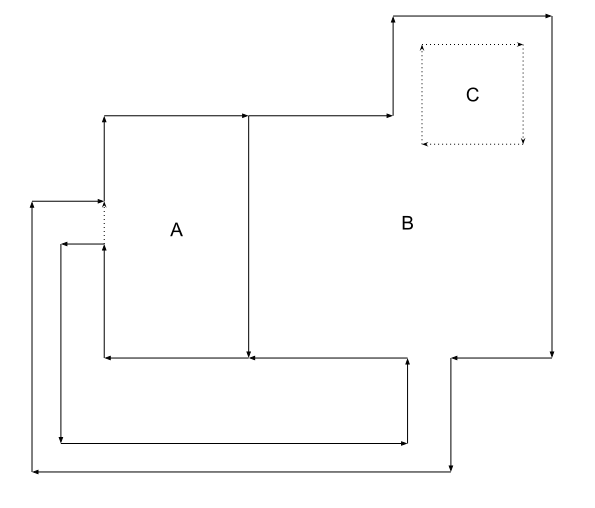
\includegraphics[width=0.8\linewidth]{linedefs_and_sectors}
	\end{center}
	
	\captionsetup{width=0.8\linewidth}
	\caption[A simple level showing sectors and linedefs]{A simple level showing three sectors A, B and C and the linedefs defining them, following the positive oriented curve constraint. Sector C can be viewed as a small platform inside the sector B. Solid arrows represent walls, while dashed lines represent invisible linedefs or changes in height between two sectors (steps). In this level, every solid arrow is a linedef that specifies only a right sidedef, with the exception of the one separating sectors A and B that has both a right and a left one.}
	\label{fig:sectors}
	\medskip
	
\end{figure}


\subsection{Conversion issues} 
Since 1994 many DOOM players started producing a large amount of levels and increasingly sophisticated editors came to light. This led to a notable variety in conventions, optimizations and use of bad practices that we tried to deal with in developing the Python module for reading and writing wad files. Some of these practices includes unnecessary lumps, random-data instead of null padding for names and other inconsistencies or arbitrary conventions. 
However, we paid particular attention during the writing phase in order to precisely follow the specifications and avoid generating low quality WAD files as much as we could.
Some other difficulties came with the necessity to render wad files as images and vice-versa. The first one is that neither \glspl{linedef} nor vertices came in an any ordered format, along with the fact that sector vertices are not explicitly defined but only referenced through the linedef/sidedef chain which means that for finding a sector shape one has to find all sidedefs with the desired sector number, than find all the linedefs referencing those sidedefs and lastly retrieving the vertices, leading to an increase of complexity. Another one is given by the fact that although sectors must be positively oriented curves, it is not mandatory to use the left sidedefs for adjacent sectors, leading to duplicated linedefs in the opposite direction. Even some optimizations such as sidedef compression may be possible, that is referencing the same sidedef wherever the same wall texture is used, adding complexity to the conversion script. Lastly, the concept of sector and the concept of room are not equivalent, since even though a sector is defined as an area of constant height this does not enforce to define a sector only where height changes, so the semantic of a sector actually depends on the designer and the editor used. 


\section{Target Data Format: Feature Maps and Vectors}
\label{sec:TargetFormat}
\paragraph{Introduction} This section provides a description of the data format as it is stored in the level dataset.
\subsection{Level Description and Motivation}
%TODO: Perché le immagini? Come mai divise così? Come mai l'encoding in questo modo?
\paragraph{}Levels are read as a structured object by a module we wrote for the purpose of providing developers and designers a programmatic way to access, analyse and edit DOOM WAD files, instead of using visual authoring software. This allows to automatise some tasks that would be very long to accomplish with standard editors or tools and also offers developers the possibility to write custom editor and scripts. \\*
In order to provide the most complete set of information possible every level is converted to a set of images, called \glspl{featuremap} in this work, a tiled representation in textual format that is an extension of the one taken from \cite{VGLC}, a graph representation and a set of textual and scalar features that contains both the \gls{WAD} meta-data and the level features and metrics calculated either on the WAD representation (sectors, subsectors, linedefs, etc), the \gls{featuremap} representation or the graph representation of the level. A detailed list and explanation of each feature is provided in section~\ref{features}. \\*
The choice of these representations have been made primarily for the need of having a data format that the generator model can work  on. In particular, convolutional neural netoworks are naturally designed to work well with bi-dimensional or tri-dimensional data such as (multi-channel) images, for this reason the image representation arose naturally. The text representation is provided mainly for consistency with the data format given in \cite{VGLC}, even if our representation uses two characters per tile instead of one. Finally, scalar and graph representation have been collected for the need of quantifying and summarising some properties and having a more abstract representation of a level, which can be very helpful in the case this data had to be used in other works.

\subsection{Feature Maps}
%TODO: Describe the maps and data encoding
\paragraph{} \glspl{featuremap} are a set of images each of them describing a different aspect of the level. In particular we used for each \gls{featuremap} a grayscale 8-bit image in which each pixel can assume values between 0 an 255. This allowed to obtain a good degree of precision while still maintaining a reasonable dataset size. \\*
Because of the motivations explained in section~\ref{par:coords}, each pixel in a \gls{featuremap} corresponds to a square of 32x32 \gls{MU}. 
In the following paragraph we will describe in detail each of them along with the data encoding.

\paragraph{\gls{floormap}} The \gls{floormap} is the most basic form of level representation, since it only represents which part of the space are occupied by the level and which are empty. This kind of map is often used in robotic mapping. \\*
This map also describes approximatively the level area that is possible to traverse, since in DOOM walls have no thickness. \\*
"Floor" pixels have value 255 (white) and "Empty" pixels have value 0 (black).

\paragraph{\gls{wallmap}} The \gls{wallmap} represent the impassable walls of the level. They are represented as a one-pixel-wide line and are obtained by directly drawing each \gls{linedef} with the impassable flag set on a black image. \\*
Pixel values are 0 for Empty area or floors and 255 for the walls.

\paragraph{\gls{heightmap}} The \gls{heightmap} is another common map used for visualizing the height of a certain surface. Since height level in DOOM levels are completely arbitrary and virtually unbounded, we normalize each level between its lowest and highest height, assigning the pixel value 0 for empty parts of the level and the remaining are calculated from the formula $ c_{h} = \lfloor h * \dfrac{255}{|H|} \rfloor $, where $ H $ is the ordered set of possible height values for the level and $ h \in \{1, 2, ..., |H| \} $ is the index of the height value in $ H $ for which we want to calculate the encoded colour. \\*
 For example if a level takes the height values $ H = \{ 0, 10, 15, 20 \} $ they will be encoded respectively as $ c_{h} = \{ 63, 127, 191, 255\} $ and 0 for the empty areas. Although this map loses the information about the differences between a height level and another, it has the advantage to represent "higher" and "lower" parts of the level without polarizing the entire map due to extreme levels: while the majority of the levels has a few changes that can be approximated as uniform (such as levels with stairs connecting a few rooms), other had some extreme changes in height but only for a small portion of the map (like a very high elevator leading to a small secret room) that led to scaling problems.
 
\paragraph{\gls{thingsmap}} The \gls{thingsmap} represent only data that is contained in the THINGS lump. It features a series of pixels placed at the thing coordinate, with a value that corresponds to a particular "thing". Pixel colours have been grouped by functional purposes so for example weapons occupies values that are close each other. This is for tolerating some output noise during generation without completely changing the functional aspect of an object as would have happened if we kept the original things encoding. Tables \ref{tab:thingsmap1}, \ref{tab:thingsmap2} and \ref{tab:thingsmap3} lists the complete encoding for the maps. Descriptions are taken from \cite{wiki:thingtypes}.

\begin{table}[b]
	\centering
	\begin{tabularx}{\textwidth}{| c | c | X | }
		\hline
		\textbf{Value} & \textbf{Functional Category} & \textbf{Thing Description} \\
		\hline
		0	& 	& Empty \\
		1	& other	& Boss Brain \\
		2	& other	& Deathmatch start \\
		3	& other	& Player 1 start \\
		4	& other	& Player 2 start \\
		5	& other	& Player 3 start \\
		6	& other	& Player 4 start \\
		7	& other	& Spawn shooter \\
		8	& other	& Spawn spot \\
		9	& other	& Teleport landing \\
		10	& keys	& Blue keycard \\
		11	& keys	& Blue skull key \\
		12	& keys	& Red keycard \\
		13	& keys	& Red skull key \\
		14	& keys	& Yellow keycard \\
		15	& keys	& Yellow skull key \\
		16	& decorations	& Bloody mess \\
		17	& decorations	& Bloody mess \\
		18	& decorations	& Candle \\
		19	& decorations	& Dead cacodemon \\
		20	& decorations	& Dead demon \\
		21	& decorations	& Dead former human \\
		22	& decorations	& Dead former sergeant \\
		23	& decorations	& Dead imp \\
		24	& decorations	& Dead lost soul (invisible) \\
		25	& decorations	& Dead player \\
		26	& decorations	& Hanging leg \\
		27	& decorations	& Hanging pair of legs \\
		28	& decorations	& Hanging victim, arms out \\
		29	& decorations	& Hanging victim, one-legged \\
		30	& decorations	& Hanging victim, twitching \\
		31	& decorations	& Pool of blood \\
		32	& decorations	& Pool of blood \\
		33	& decorations	& Pool of blood and flesh \\
		34	& decorations	& Pool of brains \\
						\hline
			\end{tabularx}
		\caption{ThingsMap Encoding (1 of 3)}
		\label{tab:thingsmap1}
		\end{table}
		
		\begin{table}[b]
			\centering
			\begin{tabularx}{\textwidth}{| c | c | X | }
				\hline
				\textbf{Value} & \textbf{Functional Category} & \textbf{Thing Description} \\
				\hline
		
		35	& obstacles	& Barrel \\
		36	& obstacles	& Burning barrel \\
		37	& obstacles	& Burnt tree \\
		38	& obstacles	& Candelabra \\
		39	& obstacles	& Evil eye \\
		40	& obstacles	& Five skulls "shish kebab" \\
		41	& obstacles	& Floating skull \\
		42	& obstacles	& Floor lamp \\
		43	& obstacles	& Hanging leg \\
		44	& obstacles	& Hanging pair of legs \\
		45	& obstacles	& Hanging torso, brain removed \\
		46	& obstacles	& Hanging torso, looking down \\
		47	& obstacles	& Hanging torso, looking up \\
		48	& obstacles	& Hanging torso, open skull \\
		49	& obstacles	& Hanging victim, arms out \\
		50	& obstacles	& Hanging victim, guts and brain removed \\
		51	& obstacles	& Hanging victim, guts removed \\
		52	& obstacles	& Hanging victim, one-legged \\
		53	& obstacles	& Hanging victim, twitching \\
		54	& obstacles	& Impaled human \\
		55	& obstacles	& Large brown tree \\
		56	& obstacles	& Pile of skulls and candles \\
		57	& obstacles	& Short blue firestick \\
		58	& obstacles	& Short green firestick \\
		59	& obstacles	& Short green pillar \\
		60	& obstacles	& Short green pillar with beating heart \\
		61	& obstacles	& Short red firestick \\
		62	& obstacles	& Short red pillar \\
		63	& obstacles	& Short red pillar with skull \\
		64	& obstacles	& Short techno floor lamp \\
		65	& obstacles	& Skull on a pole \\
		66	& obstacles	& Stalagmite \\
		67	& obstacles	& Tall blue firestick \\
		68	& obstacles	& Tall green firestick \\
		69	& obstacles	& Tall green pillar \\
		70	& obstacles	& Tall red firestick \\
		71	& obstacles	& Tall red pillar \\
		72	& obstacles	& Tall techno floor lamp \\
		73	& obstacles	& Tall techno pillar \\
		74	& obstacles	& Twitching impaled human \\
		
								\hline
	\end{tabularx}
\caption{ThingsMap Encoding (2 of 3)}
\label{tab:thingsmap2}
\end{table}

\begin{table}[b]
\centering
\begin{tabularx}{\textwidth}{| c | c | X | }
\hline
\textbf{Value} & \textbf{Functional Category} & \textbf{Thing Description} \\
\hline
		
		75	& monsters	& Arachnotron \\
		76	& monsters	& Arch-Vile \\
		77	& monsters	& Baron of Hell \\
		78	& monsters	& Cacodemon \\
		79	& monsters	& Chaingunner \\
		80	& monsters	& Commander Keen \\
		81	& monsters	& Cyberdemon \\
		82	& monsters	& Demon \\
		83	& monsters	& Former Human Trooper \\
		84	& monsters	& Former Human Sergeant \\
		85	& monsters	& Hell Knight \\
		86	& monsters	& Imp \\
		87	& monsters	& Lost Soul \\
		88	& monsters	& Mancubus \\
		89	& monsters	& Pain Elemental \\
		90	& monsters	& Revenant \\
		91	& monsters	& Spectre \\
		92	& monsters	& Spider Mastermind \\
		93	& monsters	& Wolfenstein SS \\
		94	& ammunitions	& Ammo clip \\
		95	& ammunitions	& Box of ammo \\
		96	& ammunitions	& Box of rockets \\
		97	& ammunitions	& Box of shells \\
		98	& ammunitions	& Cell charge \\
		99	& ammunitions	& Cell charge pack \\
		100	& ammunitions	& Rocket \\
		101	& ammunitions	& Shotgun shells \\
		102	& weapons	& BFG 9000 \\
		103	& weapons	& Chaingun \\
		104	& weapons	& Chainsaw \\
		105	& weapons	& Plasma rifle \\
		106	& weapons	& Rocket launcher \\
		107	& weapons	& Shotgun \\
		108	& weapons	& Super shotgun \\
		109	& powerups	& Backpack \\
		110	& powerups	& Blue armor \\
		111	& powerups	& Green armor \\
		112	& powerups	& Medikit \\
		113	& powerups	& Radiation suit \\
		114	& powerups	& Stimpack \\
		115	& artifacts	& Berserk \\
		116	& artifacts	& Computer map \\
		117	& artifacts	& Health potion \\
		118	& artifacts	& Invisibility \\
		119	& artifacts	& Invulnerability \\
		120	& artifacts	& Light amplification visor \\
		121	& artifacts	& Megasphere \\
		122	& artifacts	& Soul sphere \\
		123	& artifacts	& Spiritual armor  \\
		\hline
	\end{tabularx}
	\caption{ThingsMap Encoding (3 of 3)}
	\label{tab:thingsmap3}
\end{table}

\paragraph{\gls{triggermap}} The \gls{triggermap} is used for representing linedef triggers and the sectors which activates. Due to the vast amount of cases the doom engine can handle, only a few types of triggers have been considered. The mapping works by assigning an integer $ i \le 32 $ to every trigger object, and subdividing triggers types in 5 groups: local doors (the ones that are activable only if the players directly interact with them), remote doors, lifts, switches and teleports. Local doors can be normal or require a key of a certain colour in order to open, but they are not indexed by the trigger index since they don't require to be linked to other linedefs in order to be opened. Table~\ref{tab:triggermap} describes the encoding for each possible item $ i $.

\begin{table}[h]
\begin{tabularx}{\textwidth}{| c | c | X | }
	\hline
	\textbf{Value} & \textbf{Functional Category} & \textbf{Thing Description} \\
	\hline
	0 &	None &	Empty \\
	10 &	local doors	 & Blue key local door \\
	12 &	local doors & Red key local door \\
	14 &	local doors	 & Yellow key local door \\
	16 &	local doors & Local door \\
	32+i &	remote doors &	Remote door with tag i \\
	64+i &	lifts &	Lift with tag i \\
	128+i &	switch &	Linedef that activates the i tag \\
	192+i &	teleports &	teleport to sector i \\
	255 &	exit &	Level Exit \\
	\hline
\end{tabularx}
\caption[TriggerMap Encoding]{TriggerMap Encoding: Each item i is connected to one or more objects. For example: switch (128+1) will open the door (32+1), raise the lift (64+1), etc.}
\label{tab:triggermap}
\end{table}

\paragraph{\gls{roommap}} The \gls{roommap} represent an enumeration of the rooms obtained with an algorithm that is very similar to the morphological approach used in \citetitle{7487234}\cite{7487234}: An euclidean distance transform \cite{edt} is first applied to the \gls{floormap} obtaining a map that we call \"Distance Map\" or \"DistMap\", then the local maxima are found \cite{localmax} such that each maximum has a minimum distance of 3 from the closest one, resulting in the room center coordinates that are used as markers for a Watershed segementation \cite{watershed} using the negative distance map as basin. This results in a room segmentation that is good enough for descriptive purposes while maintaining good performances.

\subsection{Graph Representation}
Another way to represent the level is by using a graph. In particular, this graph is a region adjacency graph \cite{Trémeau00regionsadjacency} built upon the \gls{roommap}, where the nodes represent the rooms and the edges are the boundaries they have in common. This graph is built primarily for computing some features about the level and for exploiting its convenient representation of the rooms during the WAD Writing phase: this graph can be annotated with the coordinates of walls belonging to each room, and this information can be used to build a level room-by-room, with the assumption that a room could approximate a sector.


\subsection{Text Representation}
\label{textrep}
A text representation is also available, following the work of \citeauthor{VGLC} in \cite{VGLC}. In particular the representation has been extended from one character per tile/pixel to two characters. This way it has been possible to add the information about the sector tag and the damaging floor. This representation is not currently used by our work but provided for consistence with previous works. Table \ref{tab:textmap} reports all the character used for this encoding.


\begin{table}[h!]
	\begin{tabularx}{\textwidth}{| c | l | c | X | }
		\hline
		\textbf{1st character} & \textbf{Description} & \textbf{2nd Character} & \textbf{Description} \\
		\hline
		"-" &	["empty","out of bounds"] &	"-" [ascii(45)] &	Empty, no tag \\
		"X" &	["solid","wall"] &	"." [ascii(46)] &	Tag 1 \\
		"." &	["floor","walkable"] &	"/" [ascii(47)] &	Tag 2 \\
		"," &	["floor","walkable","stairs"] &	"0" [ascii(48)] &	Tag 3 \\
		"E" &	["enemy","walkable"] &	... &	... \\
		"W" &	["weapon","walkable"] &	"m" [ascii(109)] &	Tag 64 \\
		"A" &	["ammo","walkable"] &	"\textasciitilde" [ascii(126)] &	Damaging floor \\
		"H" &	["health","armor","walkable"]	 &	 & \\
		"B" &	["explosive barrel","walkable"]	 &	 & \\
		"K" &	["key","walkable"]		 & & \\
		"\textless" &	["start","walkable"]		 & & \\
		"T" &	["teleport","walkable","destination"]		 & & \\
		":" &	["decorative","walkable"]		 & & \\
		"L" &	["door","locked"]		 & & \\
		"t" &	["teleport","source","activatable"]	 &	 & \\
		"+" &	["door","walkable","activatable"]		 & & \\
		"\textgreater" &	["exit","activatable"]		 & & \\
		\hline
	\end{tabularx}
	\caption[Textual Representation Encoding]{Extended Textual Representation Encoding: A second character has been added to the one used by \citetitle{VGLC}: Each tile is expressed by two characters "XY" where X is the type of object and Y is the tag of the tile.
		Every tile that has a tag number, activates (or is activated by) the object(s) with the same tag number. 
		So, e.g. "t/" is a teleport that leads to "T/" and "X." is a switch that activates the door "+." and possibly a floor ".."}
	\label{tab:textmap}
\end{table}


	

\subsection{Scalar Features}
\label{features}
Each level is annotated with 176 numerical and textual features which are divided in four categories:
\begin{enumerate}
	\item \textbf{IDGames Archive Metadata} Contain information collected from the database when levels have been downloaded. This information contains the author, the descriptions, download urls, level title, etc. Since a WAD file can contain up to 32 levels, this information is replicated for each level found in the WAD file. \\*
	 Listed in table~\ref{tab:featureidgames}
	\item \textbf{WAD-extracted features:} This features are low-level features collected directly when processing the WAD file and include the number of lines, things, sectors, vertices, the maximum and minimum coordinates, the level size in \gls{MU} etc. \\* Listed in table~\ref{tab:featuresWAD}
	\item \textbf{PNG-extracted features} These features are computed starting from the \gls{floormap} using an Image processing library for calculating morphological properties. Each feature is calculated both directly over the whole level and as simple statistics computed over its "floors" taken singularly. A "Floor" is intended as a part of level which is not connected to the rest of the level, thus is reachable only by means of a teleporter. \\*
	Listed in tables~\ref{tab:featuresPNG1}, \ref{tab:featuresPNG2}
	\item \textbf{Graph Features} Features computed on the room graph, inspired by the work of \citeauthor{Amigoni} in \cite{Amigoni}. They are used to provide a higher level representation of the level and an indicative distribution of the different room types. \\*
	Listed in table~\ref{tab:featuresgraph}
\end{enumerate}

% TODO: Insert all the tables
\begin{table}[h!]
	\begin{tabularx}{\textwidth}{| l | X | c |}
		\hline
		\textbf{Feature Name} & \textbf{Description} & \textbf{Type} \\
		\hline
		author	&	Level Author	&	string\\
		description	&	Natural language level information	&	string\\
		credits	&	Natural language level information	&	string\\
		base	&	Natural language level information	&	string\\
		editor\textunderscore used	&	Natural language level information	&	string\\
		bugs	&	Natural language level information	&	string\\
		build\textunderscore time	&	Natural language level information	&	string\\
		rating\textunderscore value	&	doomworld.com level rating value	&	float\\
		rating\textunderscore count	&	doomworld.com vote count	&	int\\
		page\textunderscore visits	&	doomworld.com page visits	&	int\\
		downloads	&	doomworld.com download count	&	int\\
		creation\textunderscore date	&	Natural language level information	&	string\\
		file\textunderscore url	&	Download page url	&	string\\
		game	&	Doom or DoomII	&	string\\
		category	&	doomworld.com category (eg. a-z)	&	string\\
		title	&	Full level name	&	string\\
		name	&	level .zip filename	&	string\\
		path	&	relative path to wad file	&	string\\
		\hline
		
	\end{tabularx}
	\caption[ Features: IDArchive Metadata ]{ Features: IDArchive Metadata }
	\label{tab:featureidgames}
\end{table}	


\begin{table}[h!]
	\begin{tabularx}{\textwidth}{| l | X | c |}
		\hline
		\textbf{Feature Name} & \textbf{Description} & \textbf{Type} \\
		\hline
		number\textunderscore of\textunderscore lines	&	absolute number of lines in the level 	&	int \\ \hline
		number\textunderscore of\textunderscore things	&	absolute number of objects in the level	&	int \\ \hline
		number\textunderscore of\textunderscore sectors	&	absolute number of sectors (zones with same height) in the level	&	int \\ \hline
		number\textunderscore of\textunderscore subsectors	&	absolute number of subsector (convex subshapes of sectors) in the level	&	int \\ \hline
		number\textunderscore of\textunderscore vertices	&	absolute number of vertices in the level	&	int \\ \hline
		x\textunderscore max	&	maximum x coordinate	&	int \\ \hline
		y\textunderscore max	&	maximum y coordinate	&	int \\ \hline
		x\textunderscore min	&	minimum x coordinate	&	int \\ \hline
		y\textunderscore min	&	minimum y coordinate	&	int \\ \hline
		height	&	level original height in DoomUnits	&	int \\ \hline
		width	&	level original width in DoomUnits	&	int \\ \hline
		floor\textunderscore height\textunderscore [max\textbar min\textbar avg]	&	[max\textbar min\textbar avg] height for the floor	&	float \\ \hline
		ceiling\textunderscore height\textunderscore [max\textbar min\textbar avg]	&	[max\textbar min\textbar avg] height for the ceiling	&	float \\ \hline
		room\textunderscore height\textunderscore [max\textbar min\textbar avg]	&	[max\textbar min\textbar avg] difference between ceiling and floor height	&	float \\ \hline
		sector\textunderscore area\textunderscore [max\textbar min\textbar avg]	&	[max\textbar min\textbar avg] area of sectors in squadred doom map units	&	float \\ \hline
		lines\textunderscore per\textunderscore sector[max\textbar min\textbar avg]	&	[max\textbar min\textbar avg] count of sector sides	&	float \\ \hline
		aspect\textunderscore ratio	&	Ratio between the longest and the shortest dimension, since a rotation of 90° of the level does not alter playability	&	float \\ \hline
		walkable\textunderscore area	&	Number of pixels the player can walk on (nonempty\textunderscore size - walls)	&	int \\ \hline
		walkable\textunderscore percentage	&	Percentage of the level that is walkable	&	float \\ \hline
		number\textunderscore of\textunderscore \textless things\textunderscore type \textgreater	&	Total number of  \textless things\textunderscore type\textgreater in the level. \textless things\textunderscore type\textgreater: \{ artifacts, powerups, weapons, ammunitions, keys,monsters , obstacles, decorations \}	&	int \\ \hline
		\textless things\textunderscore type\textgreater\textunderscore per\textunderscore walkable\textunderscore area	&	Number of \textless things\textunderscore type\textgreater divided the walkable area in DMU. &	float \\ \hline
		start\textunderscore location\textunderscore [x\textbar y]\textunderscore px	&	[x\textbar y] coordinate (in pixels, dataset format) of the start location.	&	int \\ \hline
		slot	&	Name of the map slot. e.g "E1M1" or "MAP01"	&	string \\
		\hline
\end{tabularx}
\caption[ Features: WAD-extracted ]{ WAD-extracted features }
\label{tab:featuresWAD}
\end{table}	


\begin{table}[h!]
	\begin{tabularx}{\textwidth}{| l | X | c |}
		\hline
		\textbf{Feature Name} & \textbf{Description} & \textbf{Type} \\
		\hline
		floors	&	Number of non-connected sectors (only reachable by a teleport) of the level	&	int \\ \hline
		level\textunderscore area	&	Number of pixels composing the level	&	int \\ \hline
		floors\textunderscore area\textunderscore [mean\textbar min\textbar max\textbar std]	&	[mean\textbar min\textbar max\textbar std] number of pixels composing each floor	&	float \\ \hline
		level\textunderscore bbox\textunderscore area	&	Number of pixels of bounding box sorrounding the level	&	int \\ \hline
		level\textunderscore convex\textunderscore area 	&	Number of pixels of convex hull for the whole level	&	int \\ \hline
		floors\textunderscore convex\textunderscore area\textunderscore [mean\textbar min\textbar max\textbar std]	&	[mean\textbar min\textbar max\textbar std] Number of pixels of convex hull for each floor	&	float \textbar  int \\ \hline
		level\textunderscore eccentricity 	&	Eccentricity of the ellipse that has the same second-moments as the level. 	&	float \\ \hline
		floors\textunderscore eccentricity\textunderscore [mean\textbar min\textbar max\textbar std]	&	Eccentricity of the ellipse that has the same second-moments as each floor	&	float \\ \hline
		level\textunderscore equivalent\textunderscore diameter 	&	The diameter of a circle with the same area as the level	&	float \\ \hline
		floors\textunderscore equivalent\textunderscore diameter\textunderscore [mean\textbar min\textbar max\textbar std] 	&  [mean\textbar min\textbar max\textbar std] equivalent diameter calculated over the floors of the level	&	float \\ \hline
		level\textunderscore euler\textunderscore number 	&	Euler characteristic of the level. Computed as number of objects (= 1) subtracted by number of holes (8-connectivity).	&	int \\ \hline
		floors\textunderscore euler\textunderscore number\textunderscore [mean\textbar min\textbar max\textbar std] 	&	[mean\textbar min\textbar max\textbar std] euler number over the floors of this level	&	float\\
				\hline
	\end{tabularx}
\caption[ Features: PNG-extracted (1 of 2) ]{ PNG-extracted features (1 of 2) }
\label{tab:featuresPNG1}
\end{table}			

\begin{table}[h!]
	\begin{tabularx}{\textwidth}{| l | X | c |}
		\hline
		\textbf{Feature Name} & \textbf{Description} & \textbf{Type} \\
		\hline
		
		level\textunderscore extent 	&	Ratio of pixels in the level to pixels in the total bounding box. Non-empty size of the level.	&	float \\ \hline
		floors\textunderscore extent\textunderscore [mean\textbar min\textbar max\textbar std] 	&	[mean\textbar min\textbar max\textbar std] extent over the floors of the level	&	float \\ \hline
		level\textunderscore filled\textunderscore area 	&	Number of pixels of the level, obtained by filling the holes	&	int \\ \hline
		floors\textunderscore filled\textunderscore [mean\textbar min\textbar max\textbar std]\textunderscore mean 	&	[mean\textbar min\textbar max\textbar std] filled area over the floors of the level	&	float \\ \hline
		level\textunderscore major\textunderscore axis\textunderscore length 	&	The length of the major axis of the ellipse that has the same normalized second central moments as the level.	&	float \\ \hline
		floors\textunderscore major\textunderscore axis\textunderscore length\textunderscore [mean\textbar min\textbar max\textbar std]	&	[mean\textbar min\textbar max\textbar std] major axis length over the floors of the level	&	float \\ \hline
		level\textunderscore minor\textunderscore axis\textunderscore length 	&	The length of the minor axis of the ellipse that has the same normalized second central moments as the level	&	float \\ \hline
		floors\textunderscore minor\textunderscore axis\textunderscore length\textunderscore [mean\textbar min\textbar max\textbar std]	&	[mean\textbar min\textbar max\textbar std] minor axis length over the floors of the level	&	float \\ \hline
		level\textunderscore orientation 	&	Angle between the X-axis and the major axis of the ellipse that has the same second-moments as the level. Ranging from -pi/2 to pi/2 in counter-clockwise direction.	&	float \\ \hline
		floors\textunderscore orientation\textunderscore [mean\textbar min\textbar max\textbar std] 	&	[mean\textbar min\textbar max\textbar std] orientation over the floors of the level	&	float \\ \hline
		level\textunderscore perimeter 	&	Perimeter the level which approximates the contour as a line through the centers of border pixels using a 4-connectivity.	&	float \\ \hline
		floors\textunderscore perimeter\textunderscore [mean\textbar min\textbar max\textbar std] 	&	[mean\textbar min\textbar max\textbar std] perimeter over the floors of the level	&	float \\ \hline
		level\textunderscore solidity 	&	Ratio of pixels in the level to pixels of the convex hull image.	&	float \\ \hline
		floors\textunderscore solidity\textunderscore [mean\textbar min\textbar max\textbar std] 	&	[mean\textbar min\textbar max\textbar std] solidity over the floors of the level	&	float \\ \hline
		level\textunderscore hu\textunderscore moment\textunderscore [0 ... 6] 	&	Hu moments (translation, scale and rotation invariant).	&	float \\ \hline
		level\textunderscore centroid\textunderscore x 	&	Centroid coordinate x	&	float \\ \hline
		level\textunderscore centroid\textunderscore y 	&	Centroid coordinate y	&	float\\
		\hline
	\end{tabularx}
	\caption[ Features: PNG-extracted (2 of 2) ]{ PNG-extracted features (2 of 2) }
	\label{tab:featuresPNG2}
\end{table}			


\begin{table}[h!]
	\begin{tabularx}{\textwidth}{| l | X | c |}
		\hline
		Feature Name & Description & Type \\
		\hline
		art-points	&	Number of articulation points in the room adjacency graph. An articulation point is a node which removal would result in a bipartite graph	&	int\\
		assortativity-mean	&	Mean assortativity. Assortativity is the tendency of one node to be connected with similar nodes.	&	float\\
		betw-cen-[min \textbar  max \textbar  mean \textbar  var]	&	Node centrality statistic calculated with the betweenness method	&	float\\
		betw-cen-[skew \textbar  kurt ]	&	Node centrality statistic calculated with the betweenness method	&	float\\
		betw-cen-[Q1 \textbar  Q2 \textbar  Q3]	&	Node centrality statistic calculated with the betweenness method	&	float\\
		closn-cen-[min \textbar  max \textbar  mean \textbar  var]	&	Node centrality statistic calculated with the Closeness method	&	float\\
		closn-cen-[skew \textbar  kurt]	&	Node centrality statistic calculated with the Closeness method	&	float\\
		closn-cen-[Q1 \textbar  Q2 \textbar  Q3]	&	Node centrality statistic calculated with the Closeness method	&	float\\
		distmap-[min \textbar  max \textbar  mean ]	&	Maximum value in the distance map, i.e. the size of the largest room. Background is ignored from computation.	&	float\\
		distmap-[var \textbar  skew \textbar  kurt]	&	Mean value for the distance map, i.e. the mean room size.  Background is ignored from computation.	&	float\\
		distmap-[Q1 \textbar  Q2 \textbar  Q3]	&	Skewness of the distnace distribuiton  Background is ignored from computation.	&	float\\
		\hline
	\end{tabularx}
	\caption[ Features: Graph ]{ Graph features }
	\label{tab:featuresgraph}
\end{table}	


\section{Dataset Organization}
\label{sec:DatasetOrganization}
\subsection{Overview}
This section will describe how the dataset is stored and how it can be used for future works. \\* 
Since the dataset has been created primarily for instructing a neural network to generate new levels, the choices in data formats and data representation have been made to increase re-usability and flexibility in data manipulation. In particular the full dataset is stored first as a set of files indexed by a JSON dictionary, but for various reason that will be explained more in depth in  chapter~\ref{sec:InputSelection} in our work we only used a subset of levels stored as a separated archive.
% Full dataset ha dimensioni reali, i tfrecords sono compressi e filtrati, etc.
\subsection{Full Dataset and Filtered Dataset}
In order to keep as much information as possible from the collected levels, we structured the representation of the DOOMDataset as follow:
\begin{itemize}
	\item  A \textbf{Full Dataset} containing all the levels we collected from the Idgames Archive.
	\item A set of \textbf{Filtered Datasets} containing a subset of levels that satisfy certain constraints and which are ready to use with TensorFlow \cite{tensorflow2015-whitepaper}.
\end{itemize}
\paragraph{Full Dataset} 
 The full dataset is kept as much portable as possible, in the sense that it shouldn't need particular technologies to be accessed except the capability of parsing JSON files and NetworkX \cite{networkx} for analysing the graph structure. \\*
 It is composed of about \textbf{\textit{9460}} levels organized as a directory structure, while the maps are of different sizes given by the rescaling of the levels in \gls{MU} to tile/pixel format.\\*
 The folder is structured as follow:
 \begin{itemize}
 	\item \textbf{dataset.json} Contains all the scalar and textual information explained in section~\ref{features} and the relative paths to the files in sub-directories. Acts as a level database. 
 	\item \textbf{Original:} Contains all the WAD files as extracted by the archives downloaded from the IDGames Archive.
 	\item \textbf{Processed:} Contains the \glspl{featuremap}, the graph representation, the text representation and the relative set of features. \\*
 	Data in this folder is named as:
 	\begin{itemize}
		\item [\textbf{zipname\textunderscore WADNAME\textunderscore SLOT.json}] Is a json file containing all the features (\ref{features}) for the level.
		\item [\textbf{zipname\textunderscore WADNAME\textunderscore SLOT.networkx}] Is a gpickle compressed file containing the NetworkX graph for the level.
		\item [\textbf{zipname\textunderscore WADNAME\textunderscore SLOT.txt}] Is the Text Representation (\ref{textrep}) of the level
		\item [\textbf{zipname\textunderscore WADNAME\textunderscore SLOT\textunderscore mapname.txt}] Is the set of \glspl{featuremap} in PNG 8-bit greyscale format. 
 	\end{itemize}
 	Where zipname, wadname, mapname indicate the name of the zip archive the \gls{WAD} was stored in, the wad file itself and the \gls{featuremap} respectively, while SLOT indicates the level slot name in DOOM format (see section \ref{slotname}, "NAME" lump).
 	The choice of keeping features both in the JSON database and in separated files comes from the need of recomputing the features in an easy way (for example for adding features) and for providing the possibility to manually pick or inspect level properties without the need of accessing a long json file. This, however, comes at the cost of some data redundancy. 
 \end{itemize}


 
 \paragraph{Filtered Dataset} Due to technological limitations given by the machines used for training and other reasons explained in chapter~\ref{sec:InputSelection}, data is filtered according to some criteria in order to make them uniform in term of \gls{featuremap} size and removing some level exposing extreme values of the features. Filtered dataset is stored as a set of files described as follor:
 	\begin{itemize}
		\item \textbf{DATASETNAME-train.TFRecord} Dataset used for training the network using the TFRecord data format, which is a binary data format proposed by TensorFlow for improving data ingestion performances. 
		\item \textbf{DATASETNAME-validation.TFRecord}  Dataset used for model validation stored in TFRecord data format.
		\item \textbf{DATASETNAME.meta} Metadata and statistics about the dataset contained in train and validation datasets, in JSON format. Since the TFRecord format currently does not natively hold any information about the data contained in its records, it is useful to save data such as the item count, data structure and statistics about the dataset in a separate file, for easing the process of data normalization and other kind of operations.
 	\end{itemize}
 
 In our GitHub Repository \cite{gitrepo} it is possible to find the files relative to two different data subset:
 \begin{itemize}
 	\item \textbf{128-many-floors} Dataset of images up to 128x128 pixels (smaller levels are centered and padded) which have any number of floors, consisting of 1933 levels in training set and 829 in validation set. 
 	\item \textbf{128-one-floor} Dataset of images up to 128x128 pixels (smaller levels are centered and padded) which have just one floor, consisting of 1104 levels in training set and 474 in validation set.

 	
 \end{itemize}
	\paragraph{Provided Methods} The code repository \cite{gitrepo} hosts a Python module that provides all the necessary methods to inspect and analyse and rebuild both the full dataset and the filtered dataset. Further information is provided in the code documentation as it goes beyond the scope of this chapter.
	
\subsection{Full Dataset Statistics}

% TODO Inserire immagini distribuzioni del dataset sia di size che di features, magari in appendice
\section{Summary}
In this chapter we presented a dataset consisting of 9460 Doom Levels %TODO GO ON
	\cleardoublepage
	\chapter{System Design and Overview}
\label{ch:system_design}
\paragraph{Overview}
 This chapter describes the proposed system from an high level perspective. The purpose of this chapter is indeed to give an overview of how the system modules interact from the point of view of the use cases and data flow analysis. Section~\ref{sec:modelstructure} describes the logical structure of the generative model we use, focusing on the input and outputs and providing the notation we use for the remaining part of this work.
 Section~\ref{sec:usecases} illustrates all the main use cases for the system, highlighting how the different inputs are used to produce the expected results.
 Section~\ref{sec:dataflow} resumes the whole system design focusing on processes and data transformation rather then a component view of the system. 


\section{Generative Model Structure}
\label{sec:modelstructure}
\paragraph{Overview} The initial system design was built upon the architecture of Generative Adversarial Networks \cite{gan} from \citeauthor{gan}. Given the problem of generating video-games levels, the need to control to some extent the generation process naturally arose. For this reason, we adopted a conditional version \cite{conditionalgan} of the GAN Model, proposed by \citeauthor{conditionalgan}, applied to a more recent \gls{gan} model that is discussed in section \ref{sec:networkarch}.


\begin{figure}[h!]
	\begin{center}
		
\includegraphics[width=\linewidth]{generative_model_structure}
	\end{center}
	
	\captionsetup{width=\linewidth}
	\caption[System Overview: Generative Model Structure]{ System Overview: Generative Model Structure. A Conditional GAN is composed of a generator model and a discriminative model. The discriminative model takes as input either the Images coming from the dataset or the ones generated by the generative model. Both networks are conditioned by the Y feature vector, while the generator also takes an input a noise vector Z to sample from the data distribution it is approximating. }
	\label{fig:genmodelstructure}
\end{figure}


\paragraph{Conditional GAN Structure} We present in figure \ref{fig:genmodelstructure} the general architecture which defines the inputs and the outputs of the generative model we are using. This structure refers to the Conditional Generative Neural Network we introduced in chapter \ref{sec:introgan}. In particular, figure \ref{fig:genmodelstructure} shows the general working principles of a \gls{gan}: It is composed by two neural networks, namely a Generator and a Discriminator (or Critic, depending on the underlying architecture that is adopted). \\* The input of this subsystem are defined as follows:
\begin{itemize}
	\item $X$: Batch of images having $m$ channels, corresponding to the \glspl{featuremap}.
	\item $Y$: Batch of vectors having one component for each scalar feature considered.
	\item $Z$: Batch of random noise vector, typically sampled from a Uniform or Gaussian distribution.
\end{itemize}

The discriminator network takes as input a vector of images X and a vector of features Y, while the generator network G takes as input a the vector  Y and a vector of random noise Z, which is used to sample different points of the data distribution. We use the subscript "True" or "Gen" to distinguish from the \glspl{featuremap} coming from the input dataset and those that are generated by the generator G.
\\* For what concerns the network outputs, we have that:
\begin{itemize}
	\item  $ X_{Gen} = G(Z|Y) $: Samples generated from the generator network
	\item  $ Logits(X_{Gen}) = D(X_{Gen}|Y) $: Discriminator output when real samples are input to the discriminator.
	\item  $ Logits(X_{True}) = D(X_{True}|Y) $: Discriminator output with generated samples are provided to the discriminator.
\end{itemize}	
Logits are actually the output of the last layer of the discriminator network before the last \textit{activation function}, and they are related to the discriminator assessment of each sample. Loss functions for either the generator and the discriminator are written upon those values and alternately optimized to train the entire network. All the details are given when we'll describe the chosen GAN Architecture and the training process in section \ref{sec:networkarch}.

\section{Use Cases}
\label{sec:usecases}
\paragraph{Overview} This section will describe the main use cases of our system, which are necessary for replicating our results. The emphasis is put on how inputs and outputs are used in each case, while the internal structure of the generative model is not represented in order to simplify the notation. Every figure in this section also describes the function of the dataset metadata introduced in section \ref{sec:metadata_tfrecord} while describing the filtered dataset. In particular the neural network inputs and outputs are limited in a certain range, typically between 0 and 1 or -1 and 1. For this reason, dataset statistics are needed to properly rescale input and output data. Blocks which are written in bold type indicate those inputs and outputs that are of interest for the corresponding use case.

\subsection{Use Case: Model Optimization (Training)}
\label{sec:usecase_train}
\paragraph{} This use case describes the optimization of the model, which is commonly referred as the training phase. This is the phase in which data from the dataset is fed into the model and the loss functions are minimized in order to find the network weights that allow the generation of samples of good quality. In the ideal case the generated samples should come from a distribution which is undistinguishable from the true data distribution. In reality, this is limited by the balance of the discriminator ability in selecting features that allow it to distinguish true data from artificial one, and the generator ability in misleading the discriminator in its task by generating samples that are similar to the real ones. Figure\ref{fig:usecase_train} shows that in this use case both the Scalar Features $Y$ and the Feature Maps $X$ from the dataset are used to train the network. At each epoch the generator network is fed with a random vector $Z$ along with the conditioning vector $Y$. This procedure produces a training loss that is provided to an optimizer that acts on the network weights. 

\begin{figure}[h!]
	\begin{center}
		
\includegraphics[width=\linewidth]{use_cases_training}
	\end{center}
	
	\captionsetup{width=\linewidth}
	\caption[Use Case: Model Optimization]{Use Case: Model Optimization.}
	\label{fig:usecase_train}
\end{figure}



\subsection{Use Case: Sample Evaluation}
\label{sec:usecase_valid}
\paragraph{} This use case is useful to assess the ability of the model to generate new samples on previously unseen feature vectors and monitoring the training process. This is accomplished by running two different procedures in which only the validation set, composed of samples that are left out from the training phase, is used:
\begin{enumerate}
	\item A \textit{validation loss} is calculated by feeding the discriminator with images $X_{True, Val}$ coming from the validation set and their corresponding feature vector $Y_{Val}$. This approach is often used classical (i.e. discriminative) neural networks, where it is a good method for detecting over-fitting and assessing network generalization capabilities. In our setting, however, this may not always be a meaningful metric with every proposed underlying architecture. This is usually due to the fact that with many \gls{gan} architectures the loss does not correlate well with the quality sample. However, in section \ref{sec:networkarch} we select one of the architectures which propose to reduce the severity of this problem, among others. 
	\item  A set of \textit{quality metrics} (\ref{sec:evaluation}) are computed directly on the true samples $X_{True, Val}$ and the samples $X_{Gen, Val} = G(Z | Y_{Val}) $ generated by conditioning the network with the same features of $X_{True, Val}$. This is based on the assumption that if the network actually learns a correlation between the $Y$ vector of features and a certain set of features proper to the corresponding $X$ samples, then the true sample and the generated one might show a certain grade of similarity according to the given features. Since this may be a strong assumption, especially in the setting where we are not able to measure what features are actually mapped to each component %TODO: Cita un paper che spiega che è difficile mappare il significato delle features nelle GAN
	 $Y_i$ due to the high dimensionality of the problem, a set of more generic metrics are chosen and presented in section (\ref{sec:evaluation}). Selected metrics should be general enough to express, when averaged on batches of samples, a concept of "sample quality" without directly referring to the features encoded in the $Y$ vector.
\end{enumerate}
 Figure~\ref{fig:usecase_valid} shows how the scalar features from the validation set are used to generate new samples, that are compared to the corresponding true images.

\begin{figure}[h!]
	\begin{center}
		
\includegraphics[width=\linewidth]{use_cases_validation}
	\end{center}
	
	\captionsetup{width=\linewidth}
	\caption[Use Case: Validation and Sample Evaluation]{Use Case: Validation and Sample Evaluation.}
	\label{fig:usecase_valid}
\end{figure}

\subsection{Use Case: Sampling or Generation}
\label{sec:usecase_sampling}
\paragraph{} This use case is the one that produces new levels and it is run after a model has been trained. In particular, our system supports several methods for sampling the network in order to generate new levels. \\*
The main problem of sampling this network, as highlighted in the work of \citeauthor{slerp}\cite{slerp}, is choosing a feature vector that has lies in an area that has enough prior probability. We here present four possible methods for sampling our network, while more details are given in section \ref{sec:sampling}. These methods differ, other from the sampling method, on the input that is requested from the user. The noise vector $Z$ can be either random generated for each sampling or kept the same for testing how the $Y$ vector impacts on the network generation.

\begin{itemize}
	\item \textbf{Dataset Sampling}: This sampling method does not require any input from the user, since the conditioning vectors $Y$ are sampled from the dataset.
	\item \textbf{"Factors" Sampling}: This method allows the user to specify a set of scalars $y_{feat} = [y_1, ..., y_f] , y_i \in [0,1]$ where f is the number of features. The extrema correspond to particular values of the related feature, based on the dataset metadata. For example they can match $E[Y_{i}] \pm Std(Y_{i})$ such that each $Y_{i}$ is sampled from a region of the feature space in which it is more likely to have significant probability. This, however, may be not enough because even if the feature components $Y_{i}$ exists in the dataset distribution when taken singularly, this may not hold for their joint distribution. Moreover, the presence of the $Z$ vector greatly increase the dimensionality of the problem. That said, this method can still be useful to easily specify small perturbation in one or more features to inspect the network response, but arbitrary feature sampling remains difficult.
	\item \textbf{Direct Sampling}: This kind of sampling requires the user to directly provide a $Y$ vector as it would come from the dataset. It can be used as a starting point to develop more complex sampling methods.
	\item \textbf{"Content" Sampling}: This kind of sampling is the one that is more interesting from the perspective of an end user. If we consider a design tool that could use this network, we would need to provide the user an interface that is the most natural as possible. Rather than inspecting and "guessing" numerical values, a level designer may be interested in sketching a level and possibly obtaining a set of samples whose features reflect the ones of the provided sketch. We thus propose a sampling method that extracts the feature vector directly from a user generated image, in the same way it is extracted from the \glspl{featuremap} coming from the Dataset.
\end{itemize}
Figure~\ref{fig:usecase_sampling} shows the main differences of the proposed methods in terms of logical transformations and required inputs.

\begin{figure}[h!]
	\begin{center}
		
\includegraphics[width=\linewidth]{use_cases_generation}
	\end{center}
	
	\captionsetup{width=\linewidth}
	\caption[Use Case: Sampling or Generation]{Use Case: Sampling or Generation.}
	\label{fig:usecase_sampling}
\end{figure}




\section{Data Flow}
\label{sec:dataflow}
\begin{figure}[h!]
	\begin{center}
		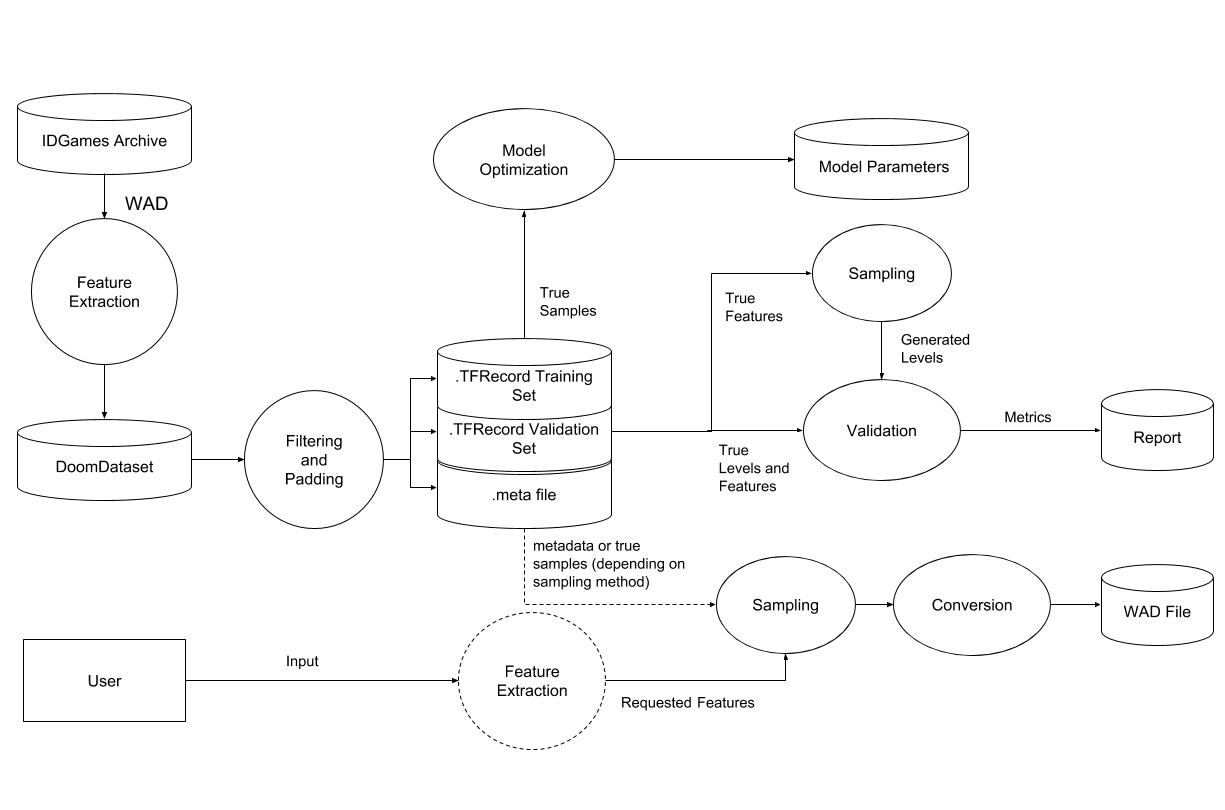
\includegraphics[width=\linewidth]{data_flow_diagram}
	\end{center}
	
	\captionsetup{width=\linewidth}
	\caption[System Overview: Data Flow Diagram]{System Overview: Data Flow Diagram. Disc-shaped blocks represent data archives, circles represent processes and transformations, while the labels on arrows represents intermediate data. Dashed lines represents objects which presence depends on the use case of reference.}
	\label{fig:dataflow}
\end{figure}

\paragraph{} Figure \ref{fig:dataflow} represent the conjunction of the use cases explained in section \ref{sec:usecases}, from a data flow perspective.  The figure is organized as a set of transformations developing from left to right. In particular, blocks on the left represent the inputs to the process and blocks on the right boundary are the produced artefacts. 
It is possible to identify three main data paths: The first produces the model parameters and it is identified with the use case "Model Optimization", or "Training" (\ref{sec:usecase_train}). \\* The second one corresponds to the Sample Evaluation use case (\ref{sec:usecase_valid}) in which levels are generated with a feature vector and then compared with the true ones corresponding to the same feature vector in the dataset. The generated metrics values are stored in a report and showed during the training phase.
The third path, which produces WAD Files, corresponds to the Sampling Use Case (\ref{sec:usecase_sampling}). In this case the data path elements depend on the sampling method used, for this reason they are indicated with dashed lines.

\newpage
\section{WAD Editor and Feature Extractor}

\section{Neural Network Architecture and Training Algorithm}
\label{sec:nn}
\paragraph{} One issue with GAN models is that the loss function is not always correlated with the generated sample quality, added to the problem of evaluating the sample quality. Although we tried some different \glspl{gan} implementations and techniques, our principal selection criterion has been the effectiveness on our particular dataset of the proposed solution in solving this stability problems.

\subsection{Network Architecture}
\label{sec:networkarch}

\subsubsection{Chosen Architecture} 
\paragraph{} Among the various \glspl{gan} implementations that are proposed in the literature, we selected the Wasserstein GAN with Gradient Penalty \cite{wgangp} (WGAN-GP) described in section~\ref{sec:wgangp} as it showed better training stability with the DCGAN layer configuration and at least comparable sample quality as opposed to the other models. We considered both the unconditional and conditional versions, by parametrizing the system upon the selected input features. The only difference with respect to the standard DCGAN model is the adoption of the \textit{sigmoid} activation function on the generator output layer instead of \textit{tanh}. This choice is motivated by the fact that tanh have been originally selected for a better color coverage in generated rgb images, while we are interested in more discrete values. This showed to help the network learning faster the representation of \glspl{floormap} and \glspl{wallmap}, while not affecting the other maps.


\subsubsection{Loss Formulation}
\paragraph{} We implement the Critic and Generator losses as in the \citetitle{wgangp} official implementation \cite{wgangp-imple}, which combines formulas \ref{eq:wganloss} and \ref{eq:gp}. Referencing to the notation introduced in \ref{sec:modelstructure} the losses are defined as follow:

\begin{equation}
\label{eq:loss}
\begin{split}
L_{Critic}^{(i)} \gets & \underbrace{\operatorname{E}(Logits(X_{Gen})) - \operatorname{E}(Logits(X_{True}))}_{\text{WGAN Loss}} + \underbrace {\lambda G_p}_{\text{Gradient Penalty}} \\
%\tag{WGAN-GP Generator Loss}
L_{Gen}^{(i)} \gets & -Logits(X_{Gen}) 
\end{split}
\end{equation}

where $X_{True}$ and $X_{Gen}$ are batches of levels sampled respectively from the dataset and the generator network, $\lambda = 10$ and $ \epsilon \sim U[0,1] $ (for the gradient penalty), in our experiments.

\paragraph{} We can now give an intuitive interpretation of the loss we used: The critic network is trained, by minimizing \ref{eq:loss}, to assign a "score" to real and generated samples. This is one of the reasons that motivate the change in name from "discriminator" to "critic"~\footnote{ Comments about the Wasserstein GAN paper from the authors of WGAN and GAN papers, among the others: \url{https://www.reddit.com/r/MachineLearning/comments/5qxoaz/r_170107875_wasserstein_gan/}}, since the network outputs are in this case not probabilities but unbound values.

\subsubsection{Training Algorithm and Hyper-Parameters}
For implementing the training algorithm we followed the algorithm suggested by \cite[alg.~1. p.~4]{wgangp}, which uses \textit{Adam}\cite{adam} as the optimizer for both the networks and optimizes $n_{critic} = 5$ times the critic network for each generator update. \\*
In addition to this implementation, we also imposed an input rotation of 90° for each sample at each epoch, such that each 4 epochs the network had in input all the possible orientation of a level. This allows us to exploit the rotation invariance in the representation of a level, since its playability is not affected by its orientation in the space it is represented. Table \ref{tab:training} shows in detail the frequency of each computation operation relative to each critic step, with reference to our TensorFlow implementation at \cite{gitrepo}. Due to implementation constraints, we calculate the Metrics out of the TensorBoard computation graph, so they appear as inputs since they have to be visualized with the other values. Reference Sample refers to the computation of a sample that is generated by the same $Y$ and $Z$ vectors, sampled at the beginning of the training phase. This helps in visualizing how the network weights optimization visually impact on the generation of one sample. \\*
The hyperparameters we used in our experiments are $\alpha=0.0002, \beta_1=0, \beta_2, \lambda=10$.

\begin{table}[h!]
	\centering
	\begin{tabularx}{\textwidth}{| c | X | X | X | X | c | X | }
		\hline
		Run Name & \multicolumn{3}{X|}{Inputs} & Outputs & Frequency & Evaluated operators \\ \cline{2-4}
		& Critic Input ($X_{True}$) & Scalar Features $(Y)$ & Generator noise (Z) &   &   &   \\
		\hline
		Train G & - & $Y_{Train}$ & $U[0,1]$ & $L_{Gen}$ & $5$ & $G_{optim}$, $summary_D$ \\ \hline
		Train D & $X_{Train}$ & $Y_{Train}$ & $U[0,1]$ & $L_{Critic}$ & $1$ & $G_{optim}$, $summary_D$\\ \hline
		Validation & $X_{Val}$ & $Y_{Val}$ & $U[0,1]$ &  $L_{Gen, Val}$, $L_{Critic, Val}$, $X_{Gen}$ & $100$ & $G_{optim}$, $summary_D$ \\ \hline
		Metrics & \multicolumn{3}{X|}{$Metrics(X_{Val}, X_{Gen})$} &  - & $100$ & $G_{optim}$, $summary_D$ \\ \hline
		Reference Sample & $-$ & $Y_{Ref}$ & $Z_{Ref}$ &  $X_{Ref}$ & $100$ & $G_{optim}$, $summary_D$ \\ \hline
		Network Checkpoint & $-$ & $-$ & $-$  & checkpoint & $100$ & $save()$ \\ \hline
	\end{tabularx}
	\caption{Training Algorithm Operations}
	\label{tab:training}
\end{table}


\subsubsection{Artefacts Reduction}
\label{sec:artefacts-reduction}
\paragraph{} One of the problem that often affects GAN is the presence of artefacts or regular patterns in the generated samples. This problem can be less noticeable when the network is generating images of real objects such in the majority of used dataset, but it's an important issue in our setting in which a change in a pixel can have noticeable impact on the resulting level and its associated metrics. This problem is well explained in \cite{artifacts} and it's due to how the transposed convolution is applied in case the kernel size is not divisible by the stride. In this case the convolution leads to an un-even overlap of outputs in the high-resolution image, generating the artefacts. Among the proposed solutions to overcome this issue we chose to simply use a kernel size of 4 and a stride of 2, which showed to reduce the problem in our case without impacting on performances or layer architecture. 

\subsection{Sample Evaluation metrics}
\label{sec:evaluation}
\paragraph{} The problem of evaluating the quality of the samples generated from a neural network remains an open area of research \cite{improved_gan}. The architectures that we considered are primarily trained on datasets consisting of images representing real objects, such as faces or bedrooms. For dealing with this problem, \citeauthor{improved_gan} propose both a process in which human annotators are asked to assess the perceived quality of the samples \cite[p.~4]{improved_gan} and the usage of the Inception Model \cite{inception} Score for assessing the perceived quality of the samples. Although many authors had success in assessing sample quality using the Inception Score, this method showed to perform poorly on our dataset. The most probable reason is that our dataset is very different from the ImageNet dataset upon which is trained the Inception Network. \\* Since tuning the Inception network to work with our dataset or applying other proposed solutions based on similarly complex models wouldn't have been possible given our computational constraints, we decided to design some heuristics that could correlate with sample quality at least with our dataset. These sample evaluation metrics give an additional measure for assessing the generated sample quality during the training process, while the final model performance is assessed by confronting the true and generated input distributions (Section \ref{sec:modelevaluation}).

\paragraph{} Instead of asking a neural network to evaluate the generated samples, our process compares two samples that have been generated by the network using the same conditioning vector. Since in principle, given a vector of scalar features $Y$, the network could generate samples which are topologically and visually very different, any metric that used quantities that are strictly related to the level topology rather than a perceived concept of "quality" couldn't lead to reasonable results. In designing these metrics we inspired to the paper \citetitle{slam}. In their work, \citeauthor{slam} propose their solution to the problem of evaluating the maps generated by a SLAM algorithm running on a mobile agent. Their approach consist in defining three metrics that capture different aspects of the analysed maps, which features some similarities with the \glspl{featuremap} we use, and considering the entire set of metrics as an approximation of the human perceived quality of a map. 
\\* Following a similar approach, we defined the following metrics for estimating the perceived quality of a sample generated by our network. These metrics are not meant to be a general solution to the problem of evaluating samples of a \gls{gan} nor to improve the work of \citeauthor{slam_metrics}, but only to be used as a quantitative tool for assessing the samples in our particular case.

\subsubsection{Entropy Mean Absolute Error}
This metric is defined as the Mean Absolute error between the entropy of two images in their colour space. In particular, since as described in chapter~\ref{sec:DatasetOrganization} we are representing maps as grey-scale images whose colour ranges between 0 and 255, we calculate the pixel distribution over each possible colour value $c$ of an image $x$, $P_{c}(x)$, then we calculate the entropy as:
\begin{equation}
S(x) = - \sum_{c=0}^{255}{ P_{c}(x) * \log{P_{c}(x)} }
\end{equation}

then, the metric over a batch of true images $X_{true}$ and a batch of generated images $X_{gen}$, both consisting of $N$ samples, is calculated as:

\begin{equation}
Entropy_{mae}(X_{true}, X_{gen}) = \frac{1}{N}\sum_{i=0}^{N-1} | S(X_{gen}(i)) - S(X_{true}(i)) |
\end{equation}

This metric is related to how different the entropy of a generated image is from the corresponding real image, which can also be interpreted as the difference in the quantity of information expressed by the two samples. In general, large values of this metric indicates that the generated sample is very noisy or the topology of the two levels are greatly different, while small values indicates that the entropy of the two images are on a comparable level. 

\subsubsection{Mean Structural Similarity Index}
This metric is defined as the Structural Similarity (SSIM) Index \cite{ssim} between two images.  This measure is the result of a framework that consider several aspects of an image, such as the luminance, the contrast and the structure, rather than basing only on a statistic. Moreover, the structural similarity technique is applied locally over the image, for reflecting the fact that pixels are more dependant on other spatially close pixels than far ones. \\*
For calculating this metric we use the implementation provided by the Scikit-Image Python library, which we leave the formulation to the paper \cite[p.~604]{ssim}, and compute the mean of the SSIM index over the images belonging to the true and generated batches. Regarding the interpretation of the metrics, values closer to 1 indicate the fact that true and generated samples are often structurally similar: in other words, the network produces samples in which the local structure of the pixels are comparable.

\subsubsection{Mean Encoding Error}
We define as "Encoding Error" a measure of how far the pixels colour of a generated image are from their closest meaningful value. Specifically, as we introduced the encoding values for each feature map in chapter~\ref{sec:DatasetOrganization} the reader might have noticed that not all values correspond an actual representation. For example, the \gls{floormap} encodes the pavement as 255 and the empty space as 0, leaving values from 1 to 254 without a real meaning. Since as highlighted in section \ref{sec:usecases} the network only reads and outputs floating point numbers between 0 and 1, this is not actually a problem of choosing an encoding space for the images, rather it is intrinsic to the network definition. Due to the generation process involving noise and non-integer parameters, the network will often output pixel colours that are in-between the possible values the input images can take, even though this behaviour decreases as the training proceeds. \\*
The definition of this function, for a generic pixel colour value $x$ which assumes meaningful values every $i$ colour values, corresponds to a periodic triangular function having base $i$ which assumes the maximum value of $1$ wherever x is halfway a meaningful value and another. More formally:

\begin{equation}
Enc_{I}(x) \equiv \sum_{k \in Z} \Lambda (\frac{2(x-kI)-I}{I})
\end{equation}


where $ \Lambda(x) $ is the unit-base triangular function such that $ \Lambda(0) = 1 $. \\*
The metric is then calculated as 

\begin{equation}
MEE(X_{gen}) = \frac{1}{N}\sum_{i=0}^{N-1} \frac{1}{|P|} \sum_{p\in P} Enc_I(p)
\end{equation}

where $p\in P$ is the colour of each pixel of the image, $|P|$ is the total number of pixels in an image and $N$ is the batch size of $X$. In particular, I is 255 for the \gls{floormap} and \gls{wallmap} while is 1 for the other maps.  \\*
Since, by construction, $MEE(X_{true}) = 0$ up to conversion errors or artefacts, this metric is only calculated for the generated samples and it is correlated with the ability of the network to represent precisely the data encoding.

\subsubsection{Mean Corner Error}
\paragraph{} This error is based on the idea introduced with the corner count metric introduced by \cite{slam}. We define our implementation of the Corner Error of two images as:
\begin{equation}
C_{err}(n_{x}, n_{y}) = \sqrt{\frac{(n_{x} - n_{y})^2}{n_{x}n_{y}}}
\end{equation}
where $n_{x}$ and $n_{y}$ are respectively the corner count of two binary images, extracted using the Harris corner detector \cite{harrisdetector}.
This formula may seem arbitrary, but it demonstrated to scale well on our dataset, since the corner count is actually limited by the size of our samples. The final metric is computed, as the other cases, averaging the corner error over the images in the batch:

\begin{equation}
MCE(X_{true}, X_{gen}) = \frac{1}{N} \sum_{i=0}^{N-1} C_{err}(n_{true,i}, n_{gen,i})
\end{equation}
Again, for simplicity, we indicated as $ n_{true,i} $ and $ n_{gen,i} $ the corner count given by \\ $ n_{i} = count(peak(harris(X_{i}))) $, with obvious meaning of the function names.
This metric is proportional to the average distance that the true and generated samples have, giving a quantitative measure of relative map complexity. It is worth nothing that it's not always the case, since generation artefacts may dramatically increase this value, producing a great number of corners. For this reason, this quantity reflects both the relative average complexity between batches of images and the presence of noise or artefacts in the generated samples.

\label{sec:editor}
\paragraph{Overview} In the previous sections of this chapter we described the generative module of the system. The module that remains to be described is the one that copes with the two endpoints of the system, in particular with the conversion from WAD to \glspl{featuremap} (or features) and vice-versa. 
\subsection{Reading and Writing}
\paragraph{Data Collection} As explained in  section~\ref{sec:DatasetOrganization}, data is hosted in an on-line archive. Due to the massive amount of levels a script for automatic download and file extraction has been written. This file also produces a preliminary JSON database, which is further expanded when WAD files are analysed.
\paragraph{Editor} The WAD parser that is provided by \citetitle{VGLC} didn't allow to extract all the features we needed for our data, while other Python modules that offered WAD file access didn't have enough documentation or support or missed features like the ability to create new files. For this reasons we proceeded to write a more complete editor, which offer the user a structured organization of the data that is contained in a WAD file using a more readable format. In particular each WAD file is read as a structured Python dictionary containing all the data we listed in chapter \ref{sec:DatasetOrganization}. The module has been realized so that a developer could ideally build a new map using only a few lines of code or even a PNG Image.


\subsection{Feature Extraction}
\paragraph{Overview} The feature extraction process is built upon our WAD Editor. In particular each WAD is first read as a structured Python dictionary, than it is processed to extract the set of features we provide with the dataset.
\paragraph{WAD to Feature Maps} The process of generating the Feature Maps is quite straightforward: For each \gls{sector} the floor height is drawn as a filled polygon on an image and the sector tags annotated. Then, each linedef is drawn as a straight line, producing the \gls{wallmap}, thus linedef triggers are matched with the relative sector tags for generating the \gls{triggermap}. \glspl{floormap} are derived by simply flattening the heightmap colour. During the process that generates the \glspl{featuremap}, the scalar features are computed on the feature maps themselves or directly from the sector and linedef data, depending on the feature. In this phase, the graph and the textual representation are also produced. 
\paragraph{Feature Maps to WAD} The WAD Editor is also able to produce WAD files from the feature map PNG representation of a level. In principle, it is possible to generate a level by  using a bitmap image editor. A more interesting use, instead, would be using this editor to write the levels generated from the network back to a WAD file, and inspect them directly in game. This is possible, at the cost of a slight loss of information due to the pixel representation of the level. In particular, line detection algorithms such as the Hough transform Line detection algorithm \cite{hough} or its probabilistic version \cite{houghprob} did not work well as expected in detecting walls from the levels generated by the network. Another approach we tried was using an edge detection algorithm for drawing sectors as contours, but this revealed to be too complex due to the way sectors are specified in WAD files (\ref{sec:WAD}). We used an alternative approach instead, exploiting the information provided by the Room Adjacency Graph built upon the \gls{roommap}: For each edge in the graph, which correspond to the boundary between a room and another, a set of walls is defined and their coordinates annotated within the graph. Approximating each sector as an entire room the process of drawing the entire map room-by-room became more straightforward. The work of inserting height changes in parts that are smaller than a room can be done by further segmenting the heightmap when considering each room and it is left as a future work.

\section{Summary} 
%TODO: Review this since some secions have been moved to this chapter
% We presented a framework for machine learning based level generation that is general enough to be used at least with any generative adversarial network 
In this chapter we presented a framework that can be used to train generative models, in particular Generative Neural Networks, to produce new levels from a previously collected dataset. In order to cope with the difficulties in sampling the network and evaluating the samples, we presented alternative methods for conditioning the network during the generation phase and for evaluating the generated samples. Moreover, we introduced our module for converting WAD levels into a set of \glspl{featuremap} and vice-versa.
	\cleardoublepage
	%\chapter{System Architecture}
\label{ch:SystemArchitecture}
\section{Component View}
\section{Neural Network Architecture}
	%\cleardoublepage
	\chapter{Experiment Design and Results}
\label{ch:experiment}

% TODO: Scrivi intro
\paragraph{}

 
\section{Neural Network Architecture and Training Algorithm}
\label{sec:nn}
\paragraph{} One issue with GAN models is that the loss function is not always correlated with the generated sample quality, added to the problem of evaluating the sample quality. Although we tried some different \glspl{gan} implementations and techniques, our principal selection criterion has been the effectiveness on our particular dataset of the proposed solution in solving this stability problems.

\subsection{Network Architecture}
\label{sec:networkarch}

\subsubsection{Chosen Architecture} 
\paragraph{} Among the various \glspl{gan} implementations that are proposed in the literature, we selected the Wasserstein GAN with Gradient Penalty \cite{wgangp} (WGAN-GP) described in section~\ref{sec:wgangp} as it showed better training stability with the DCGAN layer configuration and at least comparable sample quality as opposed to the other models.


\subsubsection{Loss Formulation}
\paragraph{} We implement the Critic and Generator losses as in the \citetitle{wgangp} official implementation \cite{wgangp-imple}, which combines formulas \ref{eq:wganloss} and \ref{eq:gp}. Referencing to the notation introduced in \ref{sec:modelstructure} the losses are defined as follow:

\begin{equation}
\label{eq:loss}
 \begin{split}
L_{Critic}^{(i)} \gets & \underbrace{\operatorname{E}(Logits(X_{Gen})) - \operatorname{E}(Logits(X_{True}))}_{\text{WGAN Loss}} + \underbrace {\lambda G_p}_{\text{Gradient Penalty}} \\
%\tag{WGAN-GP Generator Loss}
L_{Gen}^{(i)} \gets & -Logits(X_{Gen}) 
\end{split}
\end{equation}

where $X_{True}$ and $X_{Gen}$ are batches of levels sampled respectively from the dataset and the generator network, $\lambda = 10$ and $ \epsilon \sim U[0,1] $ (for the gradient penalty), in our experiments.

\paragraph{} We can now give an intuitive interpretation of the loss we used: The critic network is trained, by minimizing \ref{eq:loss}, to assign a "score" to real and generated samples. This is one of the reasons that motivate the change in name from "discriminator" to "critic"~\footnote{ Comments about the Wasserstein GAN paper from the authors of WGAN and GAN papers, among the others: \url{https://www.reddit.com/r/MachineLearning/comments/5qxoaz/r_170107875_wasserstein_gan/}}, since the network outputs are in this case not probabilities but unbound values.

\subsubsection{Training Algorithm and Hyper-Parameters}
For implementing the training algorithm we followed the algorithm suggested by \cite[alg.~1. p.~4]{wgangp}, which uses \textit{Adam}\cite{adam} as the optimizer for both the networks and optimizes $n_{critic} = 5$ times the critic network for each generator update. \\*
In addition to this implementation, we also imposed an input rotation of 90° for each sample at each epoch, such that each 4 epochs the network had in input all the possible orientation of a level. This allows us to exploit the rotation invariance in the representation of a level, since its playability is not affected by its orientation in the space it is represented. Table \ref{tab:training} shows in detail the frequency of each computation operation relative to each critic step, with reference to our TensorFlow implementation at \cite{gitrepo}. Due to implementation constraints, we calculate the Metrics out of the TensorBoard computation graph, so they appear as inputs since they have to be visualized with the other values. Reference Sample refers to the computation of a sample that is generated by the same $Y$ and $Z$ vectors, sampled at the beginning of the training phase. This helps in visualizing how the network weights optimization visually impact on the generation of one sample. \\*
 The  hyperparameters we used in our experiments are $\alpha=0.0002, \beta_1=0, \beta_2, \lambda=10$.
 


\begin{table}[h!]
	\centering
	\begin{tabularx}{\textwidth}{| c | X | X | X | X | c | X | }
		\hline
		Run Name & \multicolumn{3}{X|}{Inputs} & Outputs & Frequency & Evaluated operators \\ \cline{2-4}
		  & Critic Input ($X_{True}$) & Scalar Features $(Y)$ & Generator noise (Z) &   &   &   \\
		\hline
		Train G & - & $Y_{Train}$ & $U[0,1]$ & $L_{Gen}$ & $5$ & $G_{optim}$, $summary_D$ \\ \hline
		Train D & $X_{Train}$ & $Y_{Train}$ & $U[0,1]$ & $L_{Critic}$ & $1$ & $G_{optim}$, $summary_D$\\ \hline
		Validation & $X_{Val}$ & $Y_{Val}$ & $U[0,1]$ &  $L_{Gen, Val}$, $L_{Critic, Val}$, $X_{Gen}$ & $100$ & $G_{optim}$, $summary_D$ \\ \hline
		Metrics & \multicolumn{3}{X|}{$Metrics(X_{Val}, X_{Gen})$} &  - & $100$ & $G_{optim}$, $summary_D$ \\ \hline
		Reference Sample & $-$ & $Y_{Ref}$ & $Z_{Ref}$ &  $X_{Ref}$ & $100$ & $G_{optim}$, $summary_D$ \\ \hline
		Network Checkpoint & $-$ & $-$ & $-$  & checkpoint & $100$ & $save()$ \\ \hline
	\end{tabularx}
	\caption{Training Algorithm Operations}
	\label{tab:training}
\end{table}








\subsubsection{Artefacts Reduction}
\paragraph{} One of the problem that often affects GAN is the presence of artefacts or regular patterns in the generated samples. This problem can be less noticeable when the network is generating images of real objects such in the majority of used dataset, but it's an important issue in our setting in which a change in a pixel can have noticeable impact on the resulting level and its associated metrics. This problem is well explained in \cite{artifacts} and it's due to how the transposed convolution is applied in case the kernel size is not divisible by the stride. In this case the convolution leads to an un-even overlap of outputs in the high-resolution image, generating the artefacts. Among the proposed solutions to overcome this issue we chose to simply use a kernel size of 4 and a stride of 2, which showed to reduce the problem in our case without impacting on performances or layer architecture. 



\section{Input selection, Metrics and Sample Method}
\label{sec:input_metrics_sample}
\subsection{Input data}
\label{sec:InputSelection}
\paragraph{} For our experiments we filtered the DoomDataset by taking only the samples up to 128x128 in size and which had exactly 1 "floor". This led to a dataset of about 1000 samples, which are then augmented by rotation during the training process. This is motivated from the fact that even if the level orientation does not affect playability, using levels with more floors could lead the network to learn a correlation between floors (and how to arrange them inside the map) which could potentially be misleading or be just enforced by the sample size or the way the editor arranged them on the level coordinate space. Moreover, using only one-floor levels helped in reducing smaller artefacts that appeared as very small floors in resulting output.

\subsection{Sample Evaluation metrics}
\label{sec:evaluation}
\paragraph{} The problem of evaluating the quality of the samples generated from a neural network remains an open area of research. The architectures that we considered are primarily trained on datasets consisting of images representing real objects, such as faces or bedrooms. For dealing with this problem, \citeauthor{improved_gan} propose both a process in which human annotators are asked to assess the perceived quality of the samples \cite[p.~4]{improved_gan} and the usage of the Inception Model \cite{inception} Score for assessing the perceived quality of the samples. Although many authors had success in assessing sample quality using the Inception Score, this method showed to perform poorly on our dataset. The most probable reason is that our dataset is very different from the ImageNet dataset upon which is trained the Inception Network. \\* Since tuning the Inception network to work with our dataset or applying other proposed solutions based on similarly complex models wouldn't have been possible given our computational and time constraints, we decided to design some heuristics that could correlate with sample quality at least with our dataset. These sample evaluation metrics give an additional measure for assessing the generated sample quality during the training process, while the final model performance is assessed by confronting the true and generated input distributions (Section \ref{sec:modelevaluation}).

\paragraph{} Instead of asking a neural network to evaluate the generated samples, our process compares two samples that have been generated by the network using the same conditioning vector. Since in principle, given a vector of scalar features $Y$, the network could generate samples which are topologically and visually very different, any metric that used quantities that are strictly related to the level topology rather than a perceived concept of "quality" couldn't lead to reasonable results. In designing these metrics we inspired to the paper \citetitle{slam}. In their work, \citeauthor{slam} propose their solution to the problem of evaluating the maps generated by a SLAM algorithm running on a mobile agent. Their approach consist in defining three metrics that capture different aspects of the analysed maps, which features some similarities with the \glspl{featuremap} we use, and considering the entire set of metrics as an approximation of the human perceived quality of a map. 
\\* Following a similar approach, we defined the following metrics for estimating the perceived quality of a sample generated by our network. These metrics are not meant to be a general solution to the problem of evaluating samples of a \gls{gan} nor to improve the work of \citeauthor{slam_metrics}, but only to be used as a quantitative tool for assessing the samples in our particular case.

\subsubsection{Entropy Mean Absolute Error}
This metric is defined as the Mean Absolute error between the entropy of two images in their colour space. In particular, since as described in chapter~\ref{sec:DatasetOrganization} we are representing maps as grey-scale images whose colour ranges between 0 and 255, we calculate the pixel distribution over each possible colour value $c$ of an image $x$, $P_{c}(x)$, then we calculate the entropy as:
\begin{equation}
	S(x) = - \sum_{c=0}^{255}{ P_{c}(x) * \log{P_{c}(x)} }
\end{equation}

then, the metric over a batch of true images $X_{true}$ and a batch of generated images $X_{gen}$, both consisting of $N$ samples, is calculated as:

\begin{equation}
Entropy_{mae}(X_{true}, X_{gen}) = \frac{1}{N}\sum_{i=0}^{N-1} | S(X_{gen}(i)) - S(X_{true}(i)) |
\end{equation}

This metric is related to how different the entropy of a generated image is from the corresponding real image, which can also be interpreted as the difference in the quantity of information expressed by the two samples. In general, large values of this metric indicates that the generated sample is very noisy or the topology of the two levels are greatly different, while small values indicates that the entropy of the two images are on a comparable level. 

\subsubsection{Mean Structural Similarity Index}
This metric is defined as the Structural Similarity (SSIM) Index \cite{ssim} between two images.  This measure is the result of a framework that consider several aspects of an image, such as the luminance, the contrast and the structure, rather than basing only on a statistic. Moreover, the structural similarity technique is applied locally over the image, for reflecting the fact that pixels are more dependant on other spatially close pixels than far ones. \\*
For calculating this metric we use the implementation provided by the Scikit-Image Python library, which we leave the formulation to the paper \cite[p.~604]{ssim}, and compute the mean of the SSIM index over the images belonging to the true and generated batches. Regarding the interpretation of the metrics, values closer to 1 indicate the fact that true and generated samples are often structurally similar: in other words, the network produces samples in which the local structure of the pixels are comparable.

\subsubsection{Mean Encoding Error}
We define as "Encoding Error" a measure of how far the pixels colour of a generated image are from their closest meaningful value. Specifically, as we introduced the encoding values for each feature map in chapter~\ref{sec:DatasetOrganization} the reader might have noticed that not all values correspond an actual representation. For example, the \gls{floormap} encodes the pavement as 255 and the empty space as 0, leaving values from 1 to 254 without a real meaning. Since as highlighted in section \ref{sec:usecases} the network only reads and outputs floating point numbers between 0 and 1, this is not actually a problem of choosing an encoding space for the images, rather it is intrinsic to the network definition. Due to the generation process involving noise and non-integer parameters, the network will often output pixel colours that are in-between the possible values the input images can take, even though this behaviour decreases as the training proceeds. \\*
The definition of this function, for a generic pixel colour value $x$ which assumes meaningful values every $i$ colour values, corresponds to a periodic triangular function having base $i$ which assumes the maximum value of $1$ wherever x is halfway a meaningful value and another. More formally:

	\begin{equation}
	Enc_{I}(x) \equiv \sum_{k \in Z} \Lambda (\frac{2(x-kI)-I}{I})
	\end{equation}
	

where $ \Lambda(x) $ is the unit-base triangular function such that $ \Lambda(0) = 1 $. \\*
The metric is then calculated as 

\begin{equation}
MEE(X_{gen}) = \frac{1}{N}\sum_{i=0}^{N-1} \frac{1}{|P|} \sum_{p\in P} Enc_I(p)
\end{equation}

where $p\in P$ is the colour of each pixel of the image, $|P|$ is the total number of pixels in an image and $N$ is the batch size of $X$. In particular, I is 255 for the \gls{floormap} and \gls{wallmap} while is 1 for the other maps.  \\*
Since, by construction, $MEE(X_{true}) = 0$ up to conversion errors or artefacts, this metric is only calculated for the generated samples and it is correlated with the ability of the network to represent precisely the data encoding.

\subsubsection{Mean Corner Error}
\paragraph{} This error is based on the idea introduced with the corner count metric introduced by \cite{slam}. We define our implementation of the Corner Error of two images as:
\begin{equation}
	C_{err}(n_{x}, n_{y}) = \sqrt{\frac{(n_{x} - n_{y})^2}{n_{x}n_{y}}}
\end{equation}
where $n_{x}$ and $n_{y}$ are respectively the corner count of two binary images, extracted using the Harris corner detector \cite{harrisdetector}.
This formula may seem arbitrary, but it demonstrated to scale well on our dataset, since the corner count is actually limited by the size of our samples. The final metric is computed, as the other cases, averaging the corner error over the images in the batch:

\begin{equation}
MCE(X_{true}, X_{gen}) = \frac{1}{N} \sum_{i=0}^{N-1} C_{err}(n_{true,i}, n_{gen,i})
\end{equation}
Again, for simplicity, we indicated as $ n_{true,i} $ and $ n_{gen,i} $ the corner count given by \\ $ n_{i} = count(peak(harris(X_{i}))) $, with obvious meaning of the function names.
This metric is proportional to the average distance that the true and generated samples have, giving a quantitative measure of relative map complexity. It is worth nothing that it's not always the case, since generation artefacts may dramatically increase this value, producing a great number of corners. For this reason, this quantity reflects both the relative average complexity between batches of images and the presence of noise or artefacts in the generated samples.

\subsection{Model Evaluation}
\label{sec:modelevaluation}
\paragraph{} In order to evaluate each model performance in a systematic way we designed an experiment for comparing the distribution of true data and the one generated from the neural network, according to the features that is possible to calculate from the output images. In particular we set up two evaluation experiments: The first generates a map for each feature vector taken from the dataset and compares the distributions of the real and generated datasets, for both input features and non-input features.
The second experiment selects a subset of different maps and considers the distribution of 1000 maps that are generated using the given input feature, for each map.

\paragraph{} 
%TODO: continue this, explain more what the experiments mean



\section{Experiments}
\label{sec:experiments}
\paragraph{} We ran different input and layer settings for finding if one performed better than the others. In particular we kept fixed the WGAN-GP architecture, learning hyperparameters, the kernel size and the stride, while we varied the input features and the number of layers. \ref{tab:experiments} shows the details of each run.

\paragraph{} %TODO: Parla della selezione delle feature

\begin{table}[h!]
	\begin{tabularx}{\textwidth}{| l | c | X | X | X | X |}
		\hline
		\textbf{Run} & \textbf{Iterations} & \textbf{Features} & \textbf{Maps} & \textbf{D Layers (filters)} & \textbf{G Layers (filters)} \\
		\hline
		1 & 26000 & 
		\begin{itemize}
			\raggedright
			\small
			\item[] level equivalent diameter
			\item[] level major axis length
			\item[] level minor axis length
			\item[] level solidity
			\item[] nodes
			\item[] distmap-skew
			\item[] distmap-kurt
		\end{itemize}
		 & 
		 	\begin{itemize}
		 	\raggedright
		 	\small
		 	\item[] floormap
		 	\item[] heightmap
		 	\item[] wallmap
		 	\item[] thingsmap
		 \end{itemize}
		 & 4 (1024, 512, 256, 128) & 4 (128, 256, 512, 1024)\\
		
		\hline
		
		2 & 12000 & 
		\begin{itemize}
			\raggedright
			\small
			\item[] level equivalent diameter
			\item[] level major axis length
			\item[] level minor axis length
			\item[] level solidity
			\item[] nodes
			\item[] distmap-skew
			\item[] distmap-kurt
		\end{itemize}
		& 
		\begin{itemize}
			\raggedright
			\small
			\item[] floormap
			\item[] heightmap
			\item[] wallmap
			\item[] thingsmap
		\end{itemize}
		& 4 (1024, 512, 256, 128) & 4 (128, 256, 512, 1024)\\
		
		\hline
		
		3 & 15000 & 
		No features
		& 
		\begin{itemize}
			\raggedright
			\small
			\item[] floormap
			\item[] heightmap
			\item[] wallmap
			\item[] thingsmap
		\end{itemize}
		& 4 (1024, 512, 256, 128) & 4 (128, 256, 512, 1024)\\
		
		\hline
		
		5 & 11000 & 
		\begin{itemize}
			\raggedright
			\small
			\item[] level equivalent diameter
			\item[] level major axis length
			\item[] level minor axis length
			\item[] level solidity
			\item[] nodes
		\end{itemize}
		& 
		\begin{itemize}
			\raggedright
			\small
			\item[] floormap
			\item[] wallmap
			\item[] thingsmap
		\end{itemize}
		& 8 (1024, 1024, 512, 512, 256,  256, 128, 128) & 8 (128, 128, 256, 256, 512, 512, 1024, 1024)\\
		\hline
		
	\end{tabularx}
	\caption[ Experiments ]{ Trained models }
	\label{tab:experiments}
\end{table}	

\section{Results}
\label{sec:results}
\subsection{Resulting Model}
\label{sec:sampling}
% Alcune considerazioni su come viene campionata la rete 
% Eventuale sezione sull'interpolazione di livelli
\section{Generated Samples}
\section{In-Game Demonstration}
\section{Summary}

	\cleardoublepage
	\chapter{Conclusions and Future Work}
\label{ch:conclusions}
\paragraph{} In this chapter we make general conclusions about our work, while providing a set of open problems and the works that still have to be made. Section~\ref{sec:conclusions} reports our final conclusions, while section \ref{sec:futurework} highlights the possible future develops for enhancing our results.


\section{Conclusions}
\label{sec:conclusions}

\paragraph{} In chapter \ref{sec:results} we showed how the addition of features to the network inputs increases the quality of generated samples and leads to better learning of many features, while also providing a method to influence the network output during the sampling process. One of the most common concerns when working with GANs is that the network could overfit the training set, learning to reproduce samples from the dataset. While we cannot prove it formally, we refer to the results of \citeauthor{empiricalevaluation} in \cite[Appendix~C]{empiricalevaluation}, which claim that overfit is difficult to occur in the type of model we used, even for a small number of training samples, de facto demonstrating that the behaviour of GANs is different from that of classical deep neural networks used for classification.


\paragraph{} Although the model we designed is far for being perfect in solving the level generation problem for 2d non-linear environments such DOOM maps, we think it's still a good starting point for future improvements and could represent a viable alternative to classical Procedural Generation. In particular, most levels generated from the networks have proved to be interesting to explore and play due to the presence of particular features typical of doom maps, such as narrow tunnels and large rooms. This suggests that one of the advantages of our method with respect to Procedural Generation is that in our case there is no need of an expert designer to embed their knowledge in the generation process; still, this method allows the designer to focus on the selection of more high-level features as those we selected as network inputs. This generative method, which is commonly used to produce visually appealing images, proved to be applicable to a topological setting like ours, even if not without issues: While in creating a picture of a face, a small variation in colour intensity is quite unnoticeable and can be tolerated, in our domain even a pixel-sized difference in a level map could alter drastically the level topology itself, for example creating a new access between two areas. This issue is emphasized by the output noise which is quite common in samples generated by a GAN.

\clearpage

\section{Future Work}
\label{sec:futurework}
\paragraph{} In this section we first present the open problems we encountered in our setting, then we propose some specific works that can be made to improve our system.
\subsection{Open Problems}
\subsubsection{Data Availability}
\paragraph{} The amount of data available is a problem that affects in general every deep learning setting. As discussed in earlier chapters, the context of video-games is one of the fields in which data is less available and uniform. In our work we used a dataset of 1088 levels which have been augmented by rotation due to memory size constraints, but we envision that a larger amount of levels could make the network more accurate in generating levels. We propose a possible improvement for our system in section \ref{sec:data-augmentation}.
\subsubsection{Samples Evaluation}
\paragraph{} As we explained in section~\ref{sec:evaluation}, the problem of evaluating the samples generated by a GAN is still a recent field of research and a general prevailing model still have to be proposed. Moreover, the particular domain of our work makes even more difficult to apply the commonly used methods to assess sample quality. In section~\ref{sec:evaluation} we proposed a qualitative method for assessing the generated sample quality during the training process that works with our data. While the method we applied succeeds in indicating that the network is actually learning the level structures, the metrics we proposed have the drawback that they need to be calculated on each map differently in order to benefit of their informational power, while considered altogether for assessing the general sample quality. 

\subsubsection{Loss of accuracy}
\paragraph{} The system we designed assumes that one pixel is equivalent to 32 Doom Map Units since it's the diameter of the smallest object in DOOM. While this ensures that objects cannot overlap on the image representation, it introduces an unavoidable loss of accuracy in object positioning. Moreover, using a single pixel for representing objects such as in "Thing Maps" makes the task of distinguish generated object from noise and artefacts more difficult. While we weren't able to detect checker board artefacts in the structural maps such as the floormap, wallmap and heightmaps, the generated \glspl{thingsmap} often show an object placement that is too regular, resembling the issue discussed in section~\ref{sec:artefacts-reduction}. We envision that an increase of the dataset resolution, for example setting one pixel size to 16 MU instead of 32, would help in reducing this problem. This comes at the cost of choosing between an high resolution in representing the maps and an higher resolution in network input/output, which also allows to use more levels from the full dataset.

\subsubsection{Improving Network Sampling}
\label{sec:sampling}
\paragraph{} Due to the high dimensionality of the feature space, sampling the conditional network using arbitrary feature values often resulted in low quality samples, for this reason we sample the network around points in the feature space for which the network have been trained. However, in real applications it could be better to have the designer specify his own desired input features, such the area, the balance between large halls and corridors, etc. We envision that this issue could be reduced using more training data and possibly using soft labels as proposed by \cite{improved_gan}, at the cost of a possible increase of noise in the output. An alternative design could be the implementation of the "Content Sampling" introduced in section \ref{sec:usecase_sampling}.

\subsection{Possible Applications and future develops}
\subsubsection{Augmenting input data}
\label{sec:data-augmentation}
\paragraph{} In our work we only used levels having a single "floor", or connected figure, in order to prevent the network for learning unnecessary patterns like the position or rotation of the various floors that compose the level when they actually are irrelevant from a gameplay point of view. One method for increasing the number of training samples is re-generating the dataset considering each floor as a separated level and calculating the features on a floor basis. An additional method for using a larger part of the data we collected is to simply increase the input/output sample size, although this require more computational capabilities. 

\subsubsection{Improving samples to WAD conversion}
\paragraph{} In our work we focused on the generation process, while we also provided a simple method for playing the generated levels in DOOM. However, this method is still not perfect: only preliminary work have been done on applying the height differences in levels, and no visual improvements such as automatic texture selection have been implemented yet. Moreover, work have still to be done for decorating the level with doors, elevators and switches. 

 \subsubsection{Sample interpolation and Style Transfer}
\paragraph{} An interesting practice for generating diverse samples and assessing the generalization capabilities of the network is the interpolation of samples in the feature space \cite{slerp}. We provided a method for sampling interpolated batches of levels by providing a start and end point in feature space, while keeping the noise vector fixed. If we consider adding levels from other games to the dataset by converting them to the same domain we used, this technique can be easily used for interpolating levels from different games and study what different features they exhibit.

\subsubsection{Tweaking the model}
% Alternative models
\paragraph{} For increasing the model capabilities a lot of work can still be done. One first attempt could be tweaking the network hyperparameters in order to find a setting that allows the network to learn a better representation. Our attempts didn't find any improvements over the default settings, although we cannot prove we are using optimal values.

\subsubsection{Different architectures}
% Hybrid method based on autoencoders
\paragraph{} Due to the constant research in generative models, there is an always increasing number of different new models to try and experiment in order to improve the generation of samples. In our work we limited our search only to the mostly used pure-GAN models which could easily run on our machines, but a large number of models can still be applied.
For example, one method showing good results on faces generation that mixes GANs and Autoencoders is the BEGAN model proposed by \citeauthor{gan:BEGAN} in \cite{gan:BEGAN}. Another approach could be using high-resolution models such as in \textit{\citetitle{gan:high-res}} \cite{gan:high-res}, showing interesting improvements in visual quality by growing the generator and the discriminator progressively.

\subsubsection{Possible Applications}
The most obvious application of our work would be the case of off-line video-game level generation. In particular our work finds application whenever it is needed to obtain 3d maps which doesn't overlap on the height axis. Since this is the only particular requirement for levels to work with our framework, it is possible to extend this system to other environments and domains by just changing the feature extraction modules. In other words, the system is independent of the technology of the particular game we used for training, and it could be virtually used in any type of 3d game or simulation in which the user can move in two dimensions, eventually with changes of floor height. Possible applications in another fields could be the generation of environments for training or testing the behaviour of AI agents, and the use of the trained discriminator network for classification tasks by adding a last layer and fine tuning the resulting network. However, due to the set-up requirements currently needed for running the project, a most probable application that we envision of our work is as a starting point for the development of more complex systems or more advanced studies on Procedural Content Generation via Machine Learning applied to this type of environments.


	\cleardoublepage
	\chapter{Future Work}
\section{Open Problems}
\section{Possible Applications and future develops}

% Better map to wad conversion: Enemies, heights, textures.
% Sample interpolation
% Alternative models
% Augmenting the dataset splitting levels by floor

	\cleardoublepage
	\chapter{Appendix}
\section{Training Progress}


\section{Test Results for every feature}
\subsubsection{Input features}
\paragraph{} Tests results for the level generation in the unconditional and conditional case, for the features that have been selected as input for the conditional network are shown in table~\ref{tab:results-input-features}.
\begin{longtable}{lll}
	\caption[Test results for input features]{ \small KS-test results for input features, using a significance level of 0.05 and the Bonferroni correction method. Results are indicated with R if the null hypotesis can be rejected or with N otherwise. An asterisk indicates the network that performed better (has the minimum KS distance) if the null hypothesis is rejected in every network}\\
	\toprule
	{} & uncond & cond \\
	feature                   &        &      \\
	\midrule
	\endhead
	\midrule
	\multicolumn{3}{r}{{Continued on next page}} \\
	\midrule
	\endfoot
	
	\bottomrule
	\endlastfoot
	level\_equivalent\_diameter &      N &    N \\
	level\_major\_axis\_length   &     R* &    R \\
	level\_minor\_axis\_length   &      N &    N \\
	level\_solidity            &      R &   R* \\
	nodes                     &      R &   R* \\
	distmap-skew              &      R &   R* \\
	distmap-kurt              &      R &    N \\
	\label{tab:results-input-features}
\end{longtable}

\subsubsection{Non-Input features}
\paragraph{} Tests results for the level generation in the unconditional and conditional case, for all the features that haven't been selected as input for the conditional network are shown in table~\ref{tab:results-other-features}.

\begin{longtable}{lll}
	\caption[Test results for non input features]{ \small KS-test results for non-input features, using a significance level of 0.05 and the Bonferroni correction method. Results are indicated with R if the null hypotesis can be rejected or with N otherwise. An asterisk indicates the network that performed better (has the minimum KS distance) if the null hypothesis is rejected in every network}\\
	\toprule
	{} & uncond & cond \\
	feature                       &        &      \\
	\midrule
	\endhead
	\midrule
	\multicolumn{3}{r}{{Continued on next page}} \\
	\midrule
	\endfoot
	
	\bottomrule
	\endlastfoot
	level\_area                    &      N &    N \\
	level\_convex\_area             &      N &    N \\
	level\_eccentricity            &     R* &    R \\
	level\_euler\_number            &      R &   R* \\
	level\_extent                  &      R &   R* \\
	level\_filled\_area             &      N &    N \\
	level\_orientation             &      N &    N \\
	level\_perimeter               &      N &    N \\
	level\_hu\_moment\_0             &      N &    R \\
	level\_hu\_moment\_1             &     R* &    R \\
	level\_hu\_moment\_2             &      R &   R* \\
	level\_hu\_moment\_3             &      R &    N \\
	level\_hu\_moment\_4             &      N &    R \\
	level\_hu\_moment\_5             &      N &    R \\
	level\_hu\_moment\_6             &      R &    N \\
	level\_centroid\_x              &     R* &    R \\
	level\_centroid\_y              &     R* &    R \\
	number\_of\_artifacts           &      R &   R* \\
	number\_of\_powerups            &      R &    N \\
	number\_of\_weapons             &      R &   R* \\
	number\_of\_ammunitions         &     R* &    R \\
	number\_of\_keys                &      R &   R* \\
	number\_of\_monsters            &     R* &    R \\
	number\_of\_obstacles           &      R &   R* \\
	number\_of\_decorations         &      R &   R* \\
	walkable\_area                 &      N &    N \\
	walkable\_percentage           &      N &    N \\
	start\_location\_x\_px           &      R &   R* \\
	start\_location\_y\_px           &      R &   R* \\
	artifacts\_per\_walkable\_area   &      R &   R* \\
	powerups\_per\_walkable\_area    &      R &    N \\
	weapons\_per\_walkable\_area     &      R &   R* \\
	ammunitions\_per\_walkable\_area &     R* &    R \\
	keys\_per\_walkable\_area        &      R &   R* \\
	monsters\_per\_walkable\_area    &      R &   R* \\
	obstacles\_per\_walkable\_area   &      R &   R* \\
	decorations\_per\_walkable\_area &      R &   R* \\
	avg-path-length               &      R &   R* \\
	diameter-mean                 &      R &   R* \\
	art-points                    &     R* &    R \\
	assortativity-mean            &     R* &    R \\
	betw-cen-min                  &      N &    N \\
	betw-cen-max                  &      R &   R* \\
	betw-cen-mean                 &     R* &    R \\
	betw-cen-var                  &     R* &    R \\
	betw-cen-skew                 &      R &   R* \\
	betw-cen-kurt                 &      R &   R* \\
	betw-cen-Q1                   &     R* &    R \\
	betw-cen-Q2                   &     R* &    R \\
	betw-cen-Q3                   &     R* &    R \\
	closn-cen-min                 &     R* &    R \\
	closn-cen-max                 &      R &   R* \\
	closn-cen-mean                &     R* &    R \\
	closn-cen-var                 &      R &   R* \\
	closn-cen-skew                &     R* &    R \\
	closn-cen-kurt                &     R* &    R \\
	closn-cen-Q1                  &     R* &    R \\
	closn-cen-Q2                  &      R &   R* \\
	closn-cen-Q3                  &      R &   R* \\
	distmap-max                   &     R* &    R \\
	distmap-mean                  &     R* &    R \\
	distmap-var                   &     R* &    R \\
	distmap-Q1                    &     R* &    R \\
	distmap-Q2                    &      R &   R* \\
	distmap-Q3                    &      R &   R* \\
	\label{tab:results-other-features}
\end{longtable}

\section{KS Statistic values and corrected p-values}

\begin{longtable}{lrr}
	\caption[KS statistic values]{ \small KS statistic values for the tests. The value is correlated with the distance of the cumulative distributions of the true and generated data}\\
	\toprule
	{} &  uncond-s &    cond-s \\
	feature                       &           &           \\
	\midrule
	\endhead
	\midrule
	\multicolumn{3}{r}{{Continued on next page}} \\
	\midrule
	\endfoot
	
	\bottomrule
	\endlastfoot
	level\_area                    &  0.031279 &  0.043398 \\
	level\_convex\_area             &  0.047838 &  0.052632 \\
	level\_eccentricity            &  0.144434 &  0.223453 \\
	level\_equivalent\_diameter     &  0.031279 &  0.043398 \\
	level\_euler\_number            &  0.226311 &  0.180055 \\
	level\_extent                  &  0.127875 &  0.104340 \\
	level\_filled\_area             &  0.035879 &  0.042475 \\
	level\_major\_axis\_length       &  0.106716 &  0.116343 \\
	level\_minor\_axis\_length       &  0.076357 &  0.078486 \\
	level\_orientation             &  0.058878 &  0.068329 \\
	level\_perimeter               &  0.080957 &  0.060942 \\
	level\_solidity                &  0.121435 &  0.113573 \\
	level\_hu\_moment\_0             &  0.077277 &  0.098800 \\
	level\_hu\_moment\_1             &  0.125115 &  0.190212 \\
	level\_hu\_moment\_2             &  0.121435 &  0.104340 \\
	level\_hu\_moment\_3             &  0.106716 &  0.076639 \\
	level\_hu\_moment\_4             &  0.070837 &  0.121884 \\
	level\_hu\_moment\_5             &  0.079117 &  0.094183 \\
	level\_hu\_moment\_6             &  0.091076 &  0.059095 \\
	level\_centroid\_x              &  0.726771 &  0.777470 \\
	level\_centroid\_y              &  0.812328 &  0.815328 \\
	number\_of\_artifacts           &  0.467341 &  0.369344 \\
	number\_of\_powerups            &  0.128795 &  0.083102 \\
	number\_of\_weapons             &  0.383625 &  0.241921 \\
	number\_of\_ammunitions         &  0.359706 &  0.422899 \\
	number\_of\_keys                &  0.963201 &  0.943675 \\
	number\_of\_monsters            &  0.514259 &  0.574331 \\
	number\_of\_obstacles           &  0.519779 &  0.438596 \\
	number\_of\_decorations         &  0.823367 &  0.784857 \\
	walkable\_area                 &  0.034959 &  0.046168 \\
	walkable\_percentage           &  0.051518 &  0.081256 \\
	start\_location\_x\_px           &  0.232751 &  0.166205 \\
	start\_location\_y\_px           &  0.529899 &  0.382271 \\
	artifacts\_per\_walkable\_area   &  0.553818 &  0.390582 \\
	powerups\_per\_walkable\_area    &  0.181233 &  0.088643 \\
	weapons\_per\_walkable\_area     &  0.397424 &  0.242844 \\
	ammunitions\_per\_walkable\_area &  0.399264 &  0.444137 \\
	keys\_per\_walkable\_area        &  0.959522 &  0.938135 \\
	monsters\_per\_walkable\_area    &  0.597056 &  0.591874 \\
	obstacles\_per\_walkable\_area   &  0.665133 &  0.518006 \\
	decorations\_per\_walkable\_area &  0.897884 &  0.845799 \\
	nodes                         &  0.180313 &  0.159741 \\
	avg-path-length               &  0.174793 &  0.156048 \\
	diameter-mean                 &  0.155474 &  0.141274 \\
	art-points                    &  0.115915 &  0.139428 \\
	assortativity-mean            &  0.427032 &  0.456802 \\
	betw-cen-min                  &  0.006440 &  0.006464 \\
	betw-cen-max                  &  0.376265 &  0.347184 \\
	betw-cen-mean                 &  0.371665 &  0.384118 \\
	betw-cen-var                  &  0.362069 &  0.375894 \\
	betw-cen-skew                 &  0.250230 &  0.238227 \\
	betw-cen-kurt                 &  0.215271 &  0.207756 \\
	betw-cen-Q1                   &  0.218951 &  0.258541 \\
	betw-cen-Q2                   &  0.279669 &  0.287165 \\
	betw-cen-Q3                   &  0.301748 &  0.318560 \\
	closn-cen-min                 &  0.624655 &  0.655586 \\
	closn-cen-max                 &  0.173873 &  0.133887 \\
	closn-cen-mean                &  0.207912 &  0.213296 \\
	closn-cen-var                 &  0.314402 &  0.278856 \\
	closn-cen-skew                &  0.632935 &  0.644506 \\
	closn-cen-kurt                &  0.378105 &  0.406279 \\
	closn-cen-Q1                  &  0.201472 &  0.208680 \\
	closn-cen-Q2                  &  0.176633 &  0.169898 \\
	closn-cen-Q3                  &  0.171113 &  0.163435 \\
	distmap-max                   &  0.214351 &  0.238227 \\
	distmap-mean                  &  0.159154 &  0.202216 \\
	distmap-var                   &  0.192272 &  0.214220 \\
	distmap-skew                  &  0.152714 &  0.107110 \\
	distmap-kurt                  &  0.137994 &  0.084026 \\
	distmap-Q1                    &  0.201472 &  0.208680 \\
	distmap-Q2                    &  0.176633 &  0.169898 \\
	distmap-Q3                    &  0.171113 &  0.163435 \\
	\label{tab:results-stats}
\end{longtable}



\begin{longtable}{lrr}
	\caption[Corrected p-values]{ \small Corrected p-values using Bonferroni method}\\
	\toprule
	{} &         uncond &           cond \\
	feature                       &                &                \\
	\midrule
	\endhead
	\midrule
	\multicolumn{3}{r}{{Continued on next page}} \\
	\midrule
	\endfoot
	
	\bottomrule
	\endlastfoot
	level\_area                    &   1.000000e+00 &   1.000000e+00 \\
	level\_convex\_area             &   1.000000e+00 &   1.000000e+00 \\
	level\_eccentricity            &   3.203350e-08 &   5.274459e-22 \\
	level\_equivalent\_diameter     &   1.000000e+00 &   1.000000e+00 \\
	level\_euler\_number            &   1.051357e-22 &   1.114460e-13 \\
	level\_extent                  &   4.541127e-06 &   1.922426e-03 \\
	level\_filled\_area             &   1.000000e+00 &   1.000000e+00 \\
	level\_major\_axis\_length       &   1.060657e-03 &   1.058078e-04 \\
	level\_minor\_axis\_length       &   4.758482e-01 &   3.395852e-01 \\
	level\_orientation             &   1.000000e+00 &   1.000000e+00 \\
	level\_perimeter               &   2.148826e-01 &   1.000000e+00 \\
	level\_solidity                &   2.649796e-05 &   2.124674e-04 \\
	level\_hu\_moment\_0             &   4.074087e-01 &   6.589815e-03 \\
	level\_hu\_moment\_1             &   9.779487e-06 &   1.816326e-15 \\
	level\_hu\_moment\_2             &   2.649796e-05 &   1.922426e-03 \\
	level\_hu\_moment\_3             &   1.060657e-03 &   4.646614e-01 \\
	level\_hu\_moment\_4             &   1.000000e+00 &   2.495058e-05 \\
	level\_hu\_moment\_5             &   2.969827e-01 &   1.747566e-02 \\
	level\_hu\_moment\_6             &   3.173520e-02 &   1.000000e+00 \\
	level\_centroid\_x              &  2.720185e-250 &  1.263132e-285 \\
	level\_centroid\_y              &  4.022221e-313 &  2.723494e-314 \\
	number\_of\_artifacts           &  1.768827e-102 &   4.055502e-63 \\
	number\_of\_powerups            &   3.503463e-06 &   1.500697e-01 \\
	number\_of\_weapons             &   1.735132e-68 &   4.330549e-26 \\
	number\_of\_ammunitions         &   5.282114e-60 &   2.739392e-83 \\
	number\_of\_keys                &   0.000000e+00 &   0.000000e+00 \\
	number\_of\_monsters            &  1.874772e-124 &  4.438253e-155 \\
	number\_of\_obstacles           &  3.544692e-127 &   1.020608e-89 \\
	number\_of\_decorations         &  1.422909e-321 &  4.121210e-291 \\
	walkable\_area                 &   1.000000e+00 &   1.000000e+00 \\
	walkable\_percentage           &   1.000000e+00 &   2.092123e-01 \\
	start\_location\_x\_px           &   4.085103e-24 &   2.123218e-11 \\
	start\_location\_y\_px           &  3.028440e-132 &   9.750062e-68 \\
	artifacts\_per\_walkable\_area   &  1.297132e-144 &   8.624320e-71 \\
	powerups\_per\_walkable\_area    &   6.130510e-14 &   5.296084e-02 \\
	weapons\_per\_walkable\_area     &   1.249309e-73 &   2.653075e-26 \\
	ammunitions\_per\_walkable\_area &   2.496041e-74 &   4.829900e-92 \\
	keys\_per\_walkable\_area        &   0.000000e+00 &   0.000000e+00 \\
	monsters\_per\_walkable\_area    &  2.341589e-168 &  8.331551e-165 \\
	obstacles\_per\_walkable\_area   &  2.346143e-209 &  7.877455e-126 \\
	decorations\_per\_walkable\_area &   0.000000e+00 &   0.000000e+00 \\
	nodes                         &   8.834832e-14 &   2.130799e-10 \\
	avg-path-length               &   7.611113e-13 &   7.638737e-10 \\
	diameter-mean                 &   8.430551e-10 &   9.359119e-08 \\
	art-points                    &   1.117706e-04 &   1.650707e-07 \\
	assortativity-mean            &   5.053350e-80 &   1.523040e-90 \\
	betw-cen-min                  &   1.000000e+00 &   1.000000e+00 \\
	betw-cen-max                  &   8.086915e-66 &   1.434635e-55 \\
	betw-cen-mean                 &   3.542549e-64 &   2.070974e-68 \\
	betw-cen-var                  &   4.891902e-55 &   5.050308e-59 \\
	betw-cen-skew                 &   3.829013e-28 &   3.017244e-25 \\
	betw-cen-kurt                 &   2.227206e-20 &   8.710051e-19 \\
	betw-cen-Q1                   &   3.848983e-21 &   4.810963e-30 \\
	betw-cen-Q2                   &   1.379923e-35 &   1.804461e-37 \\
	betw-cen-Q3                   &   1.034416e-41 &   1.644635e-46 \\
	closn-cen-min                 &  1.911063e-184 &  1.371244e-202 \\
	closn-cen-max                 &   1.082671e-12 &   8.660043e-07 \\
	closn-cen-mean                &   6.820595e-19 &   6.777393e-20 \\
	closn-cen-var                 &   4.501303e-41 &   1.054396e-31 \\
	closn-cen-skew                &  2.056190e-189 &  9.669788e-196 \\
	closn-cen-kurt                &   1.760014e-66 &   9.755770e-77 \\
	closn-cen-Q1                  &   1.235166e-17 &   5.717695e-19 \\
	closn-cen-Q2                  &   3.740492e-13 &   5.455660e-12 \\
	closn-cen-Q3                  &   3.081734e-12 &   5.768903e-11 \\
	distmap-max                   &   3.438308e-20 &   3.017244e-25 \\
	distmap-mean                  &   2.362809e-10 &   1.046636e-17 \\
	distmap-var                   &   6.608149e-16 &   4.399457e-20 \\
	distmap-skew                  &   2.146329e-09 &   1.012498e-03 \\
	distmap-kurt                  &   2.362741e-07 &   1.267447e-01 \\
	distmap-Q1                    &   1.235166e-17 &   5.717695e-19 \\
	distmap-Q2                    &   3.740492e-13 &   5.455660e-12 \\
	distmap-Q3                    &   3.081734e-12 &   5.768903e-11 \\
	\label{tab:results-pvalues}
\end{longtable}


\section{Graphical results for non-input features}
\paragraph{} We omit results for features that are not informative in our specific context such as features calculated on floor basis, since the dataset we used only consisted on one-floor levels and they would match the corresponding level based features.



	\cleardoublepage
	\newglossaryentry{WAD}
{
  name=WAD,
  description={Default format of package files for the DOOM / DOOM II video-games. "WAD" is an acronym for "Where's all the Data?" \cite{wadmeaning} },  plural=WADs
}
\newglossaryentry{lump}
{
	name=Lump,
	description={ Any section of data within a \gls{WAD} file. }
}
\newglossaryentry{thing}
{
	name=Thing,
	description={ Any deployable asset of a DOOM level, such as Enemies, Power-Ups, Weapons, Decorations, Spawners, Etc. }
	plural=Things
}
\newglossaryentry{sector}
{
	name=Sector,
	description={A Sector in a DOOM level is any closed area (with possibly invisible walls) that has a constant floor and ceiling height and texture.  }
	plural=Things
}
\newglossaryentry{deathmatch}
{
	name=Deathmatch,
	description={ Game mode in which two or more players compete against each other in achieving the highest number of kills before a timeout or a player reaches a predetermined score. }
}

\newglossaryentry{MU}{
	name=MU,
	description={Map Units, Coordinate unit used in Doom Rendering Engine. }
}

\newglossaryentry{DU}{
	name=DU,
	description={Doom Units, see \gls{MU} }
}

\newglossaryentry{linedef}{
	name=Linedef,
	description={ Line that connects two vertices in the WAD file specification }
}

\newglossaryentry{sidedef}{
	name=Sidedef,
	description={ A "vertical plane" in the WAD file specification.}
}

\newglossaryentry{featuremap}{
	name=Feature Map,
	description={Image describing a particular aspect of a level},
	plural={Feature Maps}
}

\newglossaryentry{floormap}{
	name=FloorMap,
	description={Image describing which parts of the map are occupied by a floor and which are empty.}
}
\newglossaryentry{heightmap}{
	name=HeightMap,
	description={Image describing the floor height of a level}
}
\newglossaryentry{roommap}{
	name=RoomMap,
	description={Image describing the room segmentation of the level}
}
\newglossaryentry{thingsmap}{
	name=ThingsMap,
	description={Image describing how the game objects are placed inside the level}
}
\newglossaryentry{triggermap}{
	name=TriggerMap,
	description={Image describing doors, lifts and switches and their correlation}
}
\newglossaryentry{wallmap}{
	name=WallMap,
	description={Image describing the impassable walls in a level}
}
\newglossaryentry{floor}{
	name=floor,
	description={Unconnected piece of level, reachable only by means of a teleporter}
}






	\glsaddall
	\printglossaries
	\cleardoublepage
	\printbibliography
	\cleardoublepage
	
	
\end{document}